\documentclass[11pt,a4paper]{article}
\usepackage[margin=2.1cm]{geometry}
\usepackage{booktabs,xcolor,hyperref,enumitem,graphicx,float}
\setlist{itemsep=1pt,topsep=2pt}
\title{The two clocks, eight issuers}
\author{FundamentalQuantmental, HY Analyst, methodology Section 4.7}
\date{Filings as known on 18 September 2026}
\begin{document}
\maketitle
\noindent\fcolorbox{gray}{gray!6}{\parbox{\dimexpr\linewidth-2\fboxsep-2\fboxrule}{\sloppy%
\textbf{How to read this.} Each page puts what the issuer owes each year (rent, debt, interest, purchase commitments) against what pays for it.
Two issuers disclose a large signed contract book (CRWV, ORCL): their green line is contract cash. The others do not: their green line is today's EBITDAR held flat. That line is not a promise; it asks how much of today's earnings the fixed charges take.

\smallskip
\textbf{The one number to compare across all eight:} fixed charges in years of today's EBITDAR. HCA needs 3.8 years; CRWV needs 18.2.}}

\begin{center}\small
\begin{tabular}{@{}lrrrrr@{}}\toprule
Issuer & Fixed charges & Centre (years) & Years of EBITDAR & Breakeven margin & Renewal-dependent \\\midrule
CRWV & \$106bn & 5.5 & 18.2 & 1.03 & 31\% \\
ORCL & \$549bn & 8.2 & 13.9 & 0.83 & 37\% \\
HCA & \$59bn & 4.4 & 3.8 & -- & -- \\
THC & \$18bn & 3.3 & 4.2 & -- & -- \\
CCL & \$51bn & 4.7 & 6.9 & -- & -- \\
NCLH & \$18bn & 5.6 & 6.5 & -- & -- \\
MGM & \$59bn & 12.2 & 12.5 & -- & -- \\
WYNN & \$17bn & 5.9 & 9.3 & -- & -- \\
\bottomrule
\end{tabular}
\end{center}

\textbf{Changes against the first CoreWeave and Oracle note.} This run derives every input from the filings. CoreWeave's interest rate is the cash rate from the loader (4\%) instead of the hand-entered 9\%, and its contract timing comes from the 10-Q text (months 25 to 48, then 49 to 78). Its breakeven margin moves from 1.08 to 1.03 and its renewal-dependent share from 24\% to 31\%.

\textbf{Fallbacks used.} HCA tags a debt schedule that is short of its balance-sheet debt; the missing amount is put in ``thereafter''. Tenet discloses signed revenue below one year of sales, so its contract clock is treated as immaterial. Leases that run past 25 years are summed into the last bar, which is hatched.
\newpage
\section*{The macro paths behind every scenario page}
Phase expansion (from the F6 indicators with data). Sources: SPF, FOMC SEP, Treasury forwards, TRACE high yield level (168 bp).
\begin{center}\small
\begin{tabular}{@{}lrrrrr@{}}\toprule
Path & Probability & GDP (avg) & Policy rate, 2 years & 10y yield, 2 years & HY spread (bp) \\\midrule
soft landing & 86\% & 2.5\% & 3.9\% & 5.2\% & 142 \\
recession & 2\% & -0.0\% & 2.6\% & 3.0\% & 369 \\
higher for longer & 8\% & 2.2\% & 5.5\% & 5.9\% & 168 \\
disinflation rally & 4\% & 2.8\% & 2.1\% & 4.6\% & 110 \\
stagflation & 0\% & -0.1\% & 4.4\% & 3.9\% & 376 \\
\bottomrule
\end{tabular}
\end{center}
\newpage

\section{CoreWeave (CRWV), filing of 2026-06-30}
\begin{figure}[H]\centering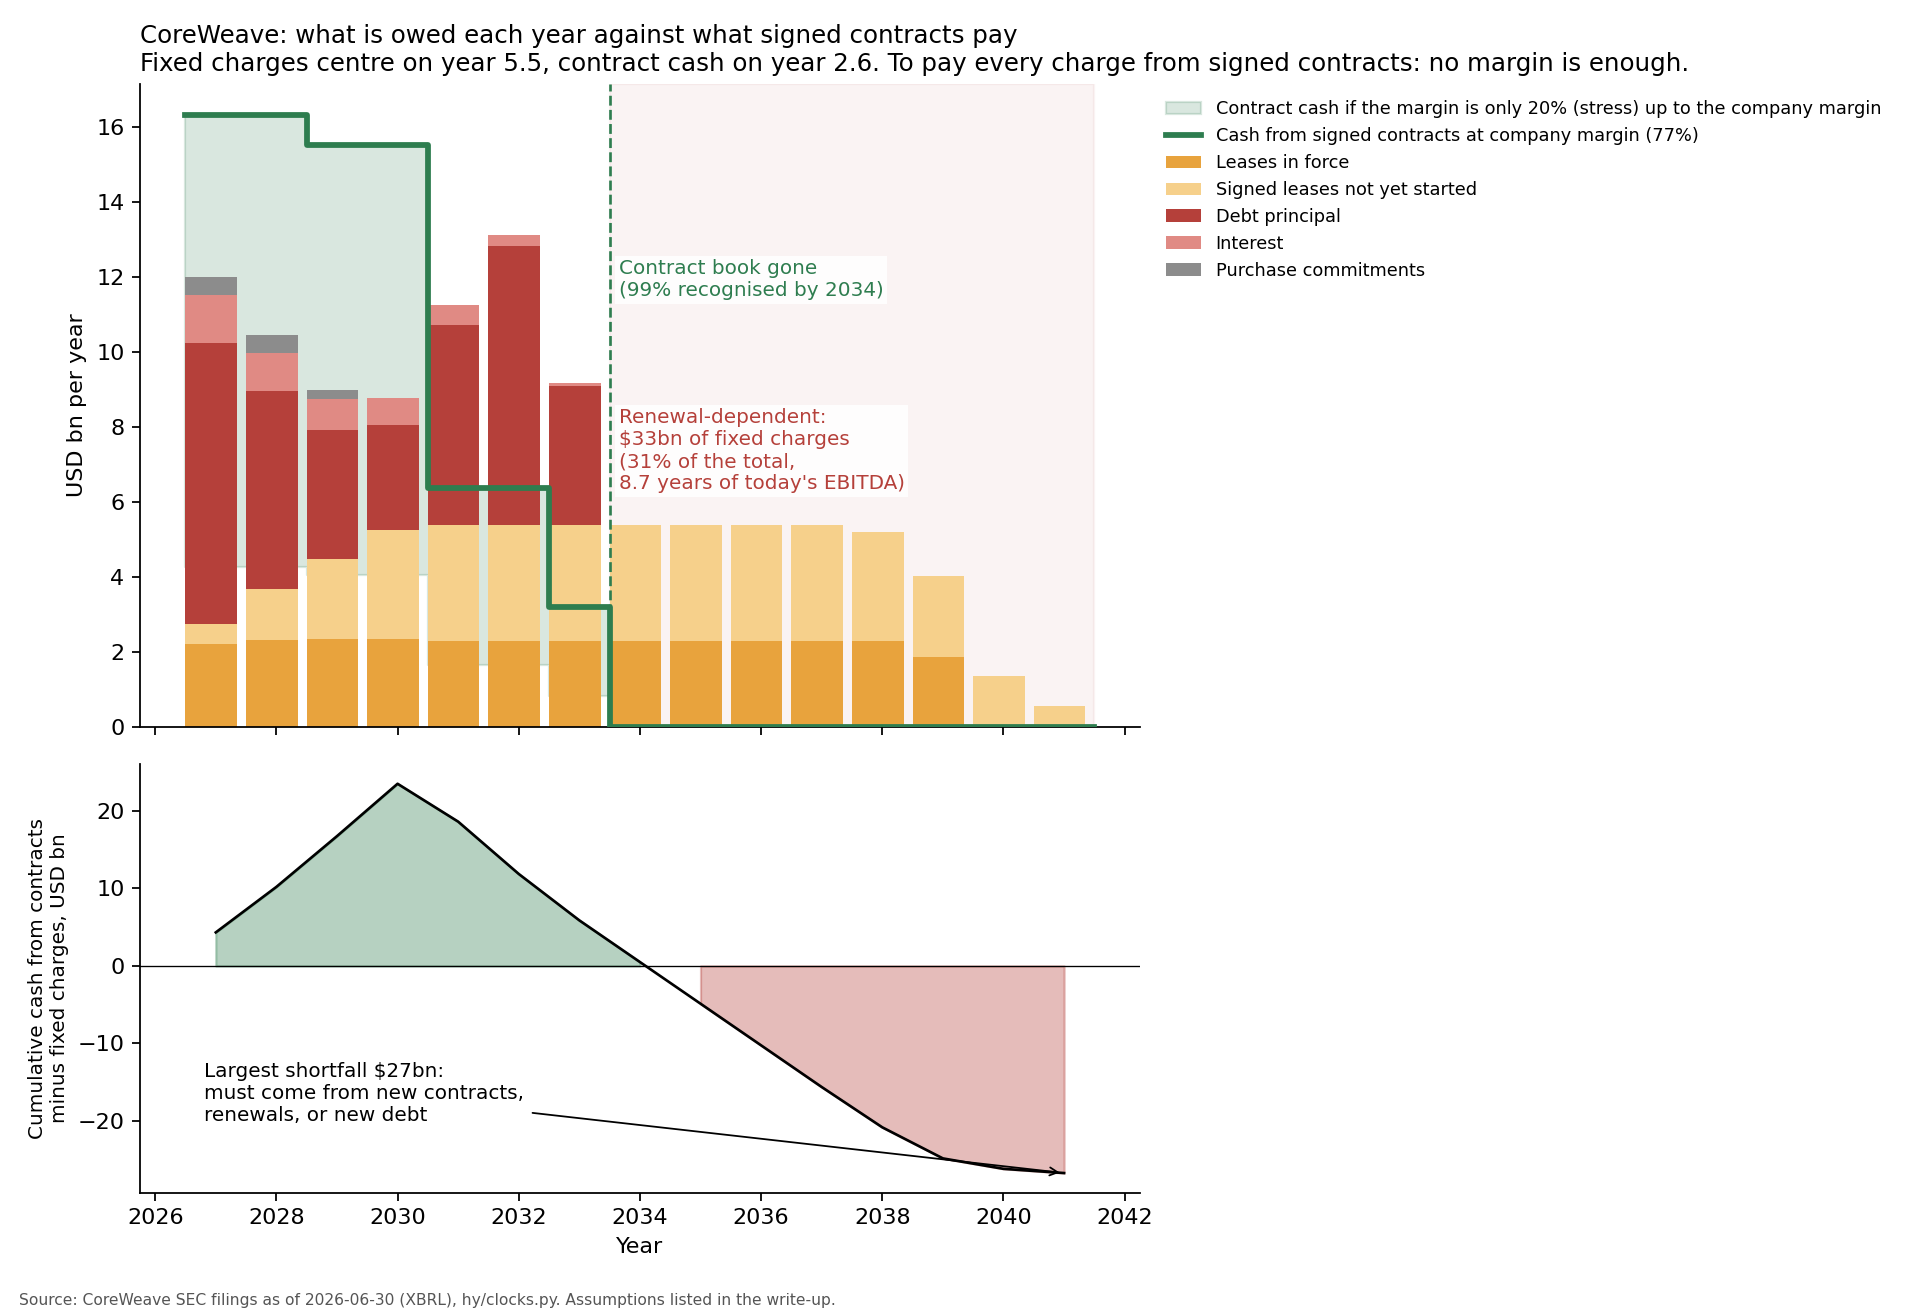
\includegraphics[width=\linewidth]{figures/clocks_all_CRWV.png}\end{figure}
\begin{itemize}
\item \textbf{Fixed charges:} \$106bn, centred on year 5.5. That is 18.2 years of today's EBITDAR.
\item \textbf{Signed contracts:} \$104bn. Breakeven margin 1.03 (no margin is enough).
\item \textbf{Renewal bet:} 31% of charges (\$33bn) fall due after the contracts end; 4.1 years of current revenue must be signed to pay them.
\item \textbf{Debt schedule:} ladder as filed; balance-sheet debt 35,551 (tag DebtInstrumentCarryingAmount).
\end{itemize}\newpage
\section*{CoreWeave (CRWV): scenarios under each macro path}
\begin{figure}[H]\centering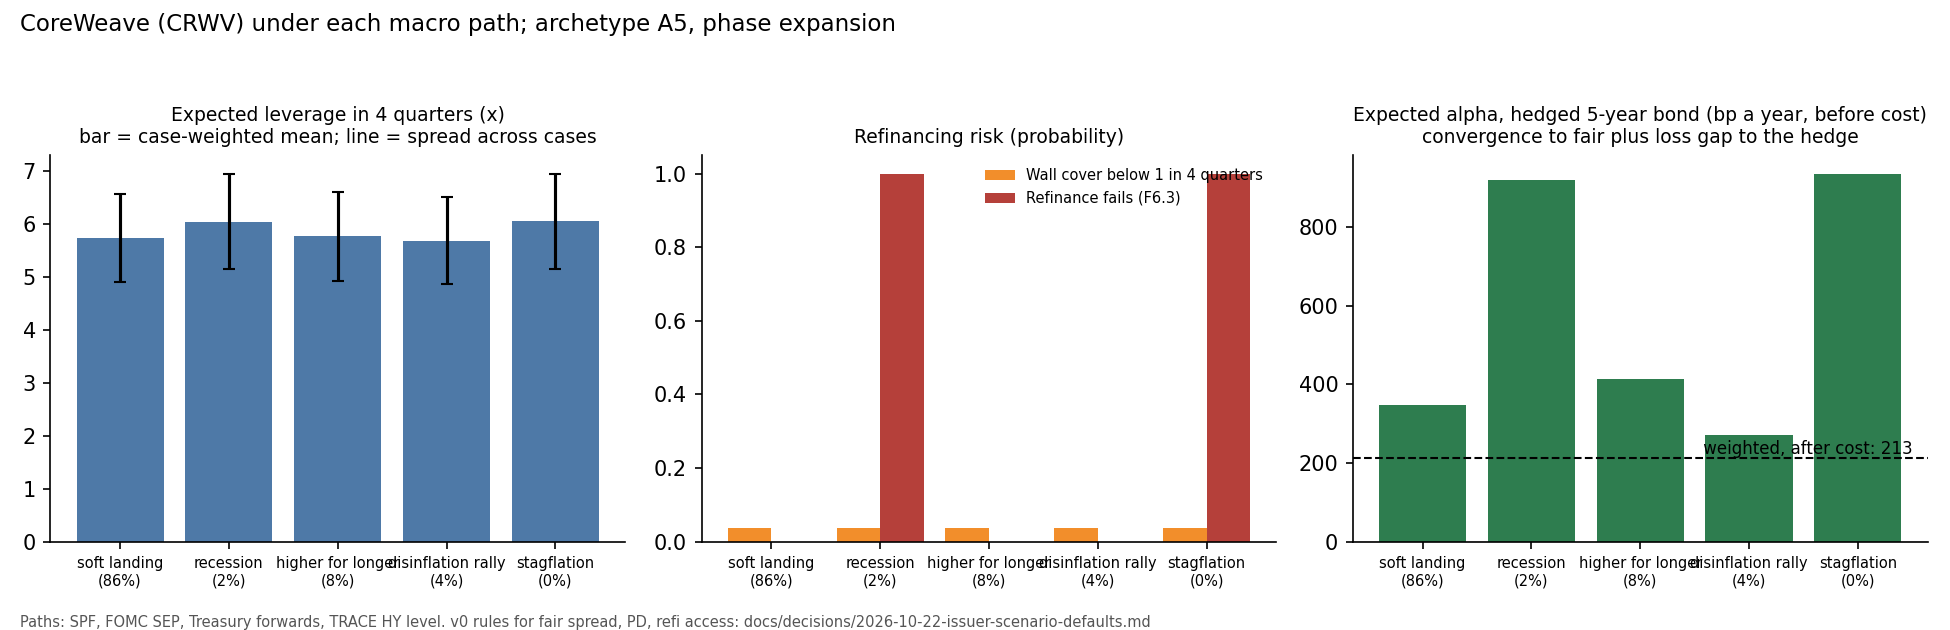
\includegraphics[width=\linewidth]{figures/scenarios_CRWV.png}\end{figure}
\begin{center}\footnotesize\setlength{\tabcolsep}{4pt}
\begin{tabular}{@{}lrrrrrrrr@{}}\toprule
Path & Prob. & Lev. 4q & Peak lev. (down) & F4 score & Wall risk & Refi fails & PD 12m & Alpha (bp/yr) \\\midrule
soft landing & 86\% & 5.7x & 9.3x & 3 & 4\% & 0\% & 4.0\% & +361 \\
recession & 2\% & 6.0x & 9.9x & 1 & 4\% & 100\% & 10.0\% & +951 \\
higher for longer & 8\% & 5.8x & 9.3x & 2 & 4\% & 0\% & 4.7\% & +428 \\
disinflation rally & 4\% & 5.7x & 9.3x & 3 & 4\% & 0\% & 3.1\% & +280 \\
stagflation & 0\% & 6.1x & 9.9x & 1 & 4\% & 100\% & 10.2\% & +968 \\
\bottomrule
\end{tabular}
\end{center}
\begin{itemize}
\item \textbf{Weighted expected alpha}, hedged 5-year bond, 6-month horizon: +376 bp a year before cost, +226 bp after a 20 bp bid-ask round trip. Framework F9 G3 (alpha after cost above zero): passes.
\item \textbf{Inputs}: archetype A5; 5-year spread 739 bp against a fair 574 bp (pair report fair line); starting growth 8.0\% a quarter; 10,597 of 35,551 (USD m) of debt due inside 8 quarters. F4 points held on every path: recent raise.
\item \textbf{Read with care}: fair spread, default probability, and refinance access follow the v0 rules of \texttt{docs/decisions/2026-10-22-issuer-scenario-defaults.md}. Under spread-proportional pricing a mispricing scales with the market, so the stress paths enlarge it; real stress often widens a gap before it closes.
\end{itemize}
\newpage
\section{Oracle (ORCL), filing of 2026-08-31}
\begin{figure}[H]\centering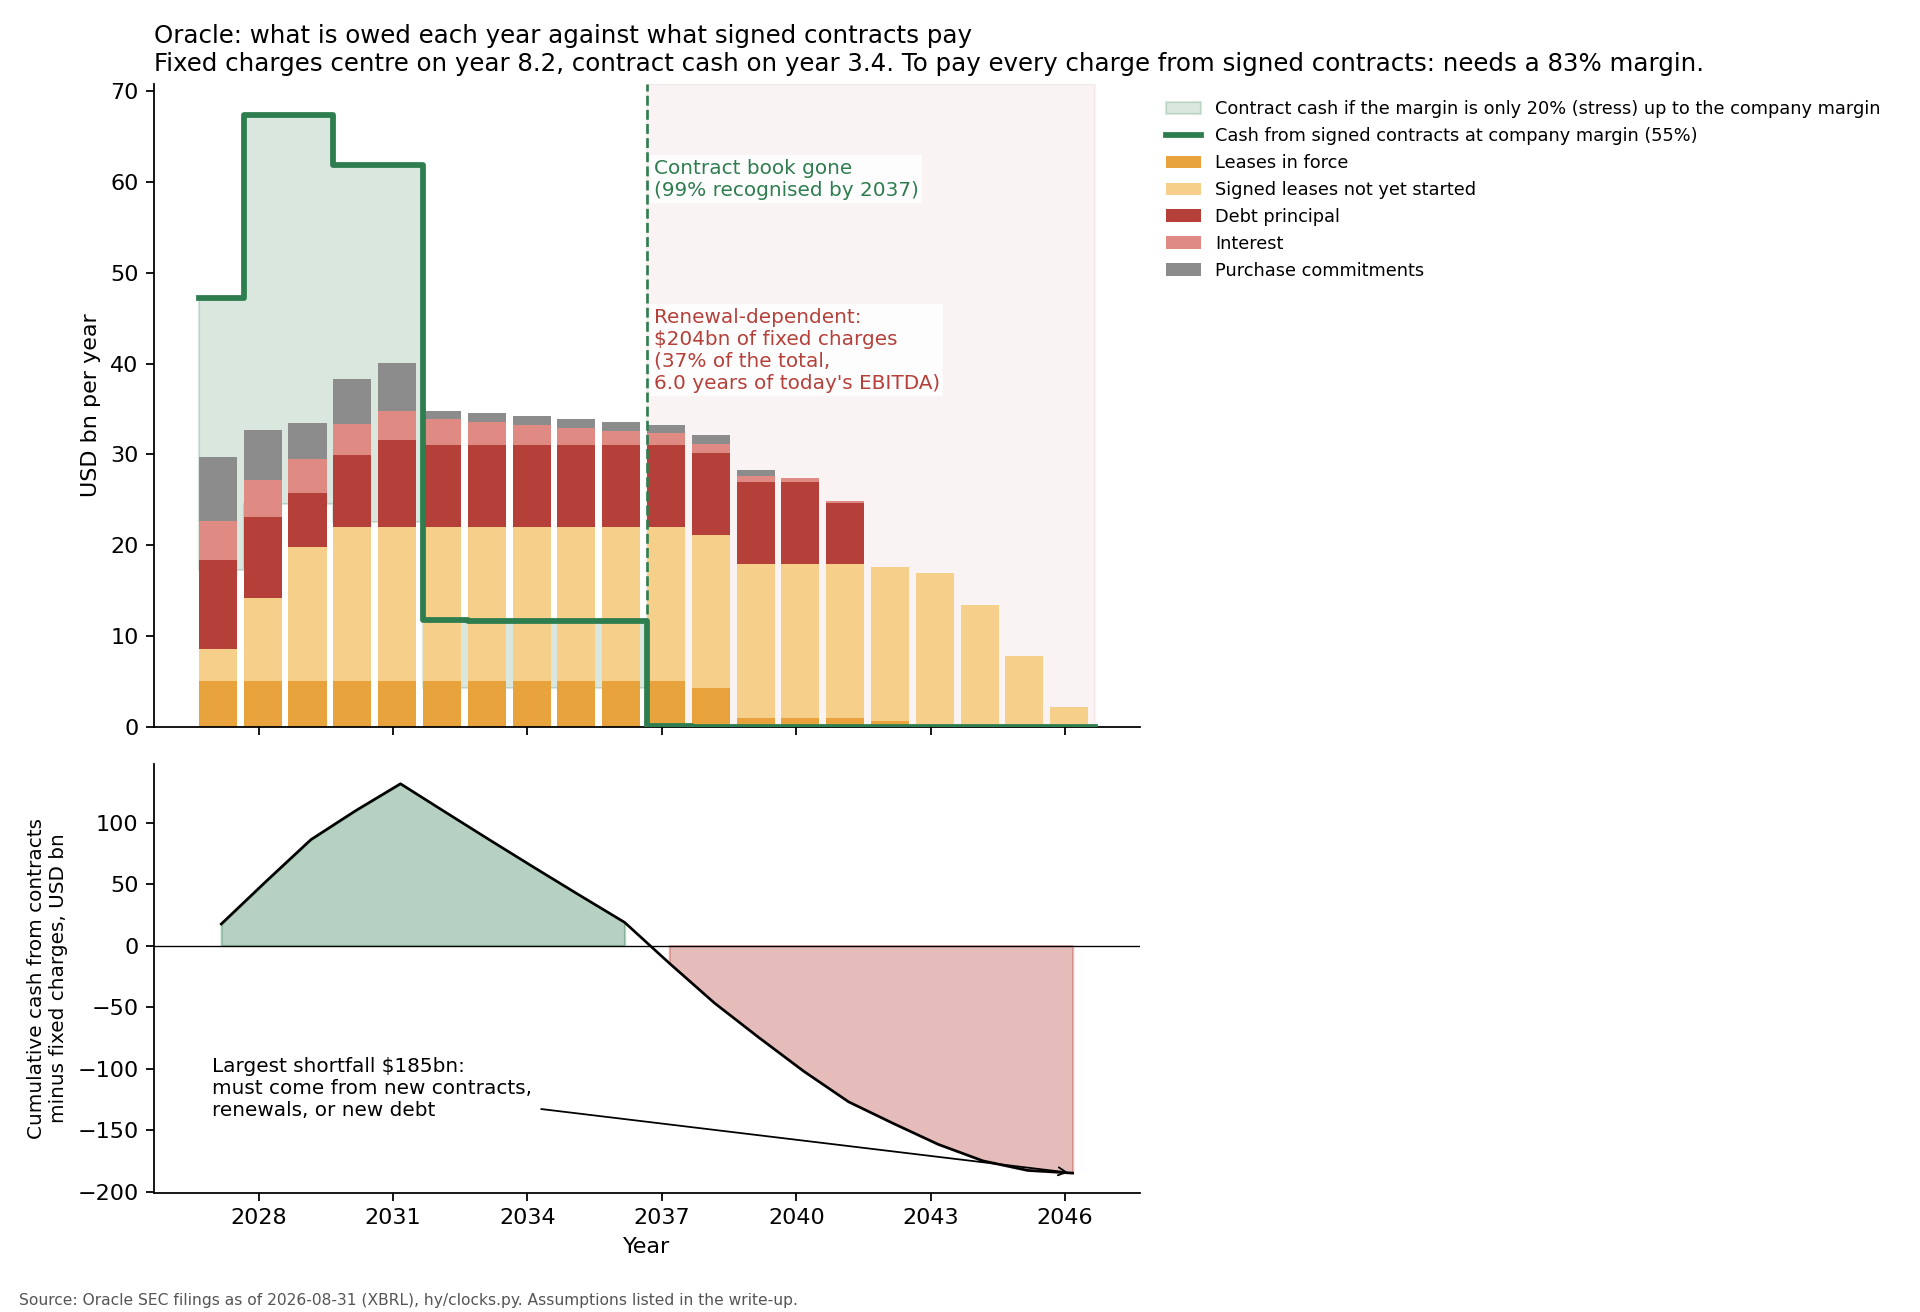
\includegraphics[width=\linewidth]{figures/clocks_all_ORCL.png}\end{figure}
\begin{itemize}
\item \textbf{Fixed charges:} \$549bn, centred on year 8.2. That is 13.9 years of today's EBITDAR.
\item \textbf{Signed contracts:} \$664bn. Breakeven margin 0.83 against a company margin of 55%.
\item \textbf{Renewal bet:} 37% of charges (\$204bn) fall due after the contracts end; 4.8 years of current revenue must be signed to pay them.
\item \textbf{Debt schedule:} ladder as filed; balance-sheet debt 125,337 (tags NotesPayableCurrent + LongTermNotesAndLoans).
\end{itemize}\newpage
\section*{Oracle (ORCL): scenarios under each macro path}
\begin{figure}[H]\centering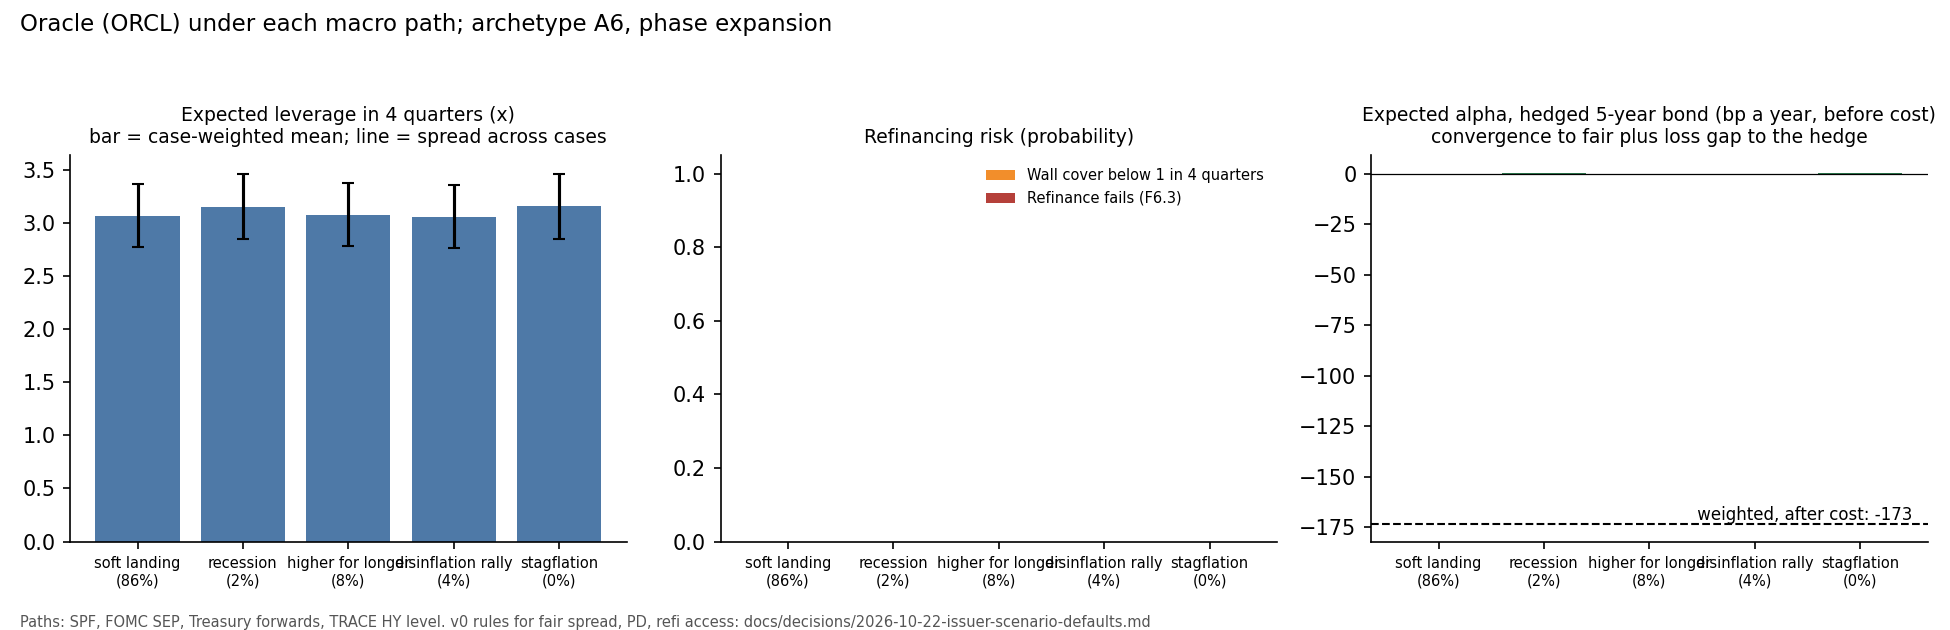
\includegraphics[width=\linewidth]{figures/scenarios_ORCL.png}\end{figure}
\begin{center}\footnotesize\setlength{\tabcolsep}{4pt}
\begin{tabular}{@{}lrrrrrrrr@{}}\toprule
Path & Prob. & Lev. 4q & Peak lev. (down) & F4 score & Wall risk & Refi fails & PD 12m & Alpha (bp/yr) \\\midrule
soft landing & 86\% & 3.1x & 4.3x & 3 & 0\% & 0\% & 0.9\% & +3 \\
recession & 2\% & 3.2x & 4.4x & 2 & 0\% & 0\% & 2.4\% & +10 \\
higher for longer & 8\% & 3.1x & 4.3x & 3 & 0\% & 0\% & 1.1\% & +4 \\
disinflation rally & 4\% & 3.1x & 4.2x & 3 & 0\% & 0\% & 0.7\% & +3 \\
stagflation & 0\% & 3.2x & 4.4x & 2 & 0\% & 0\% & 2.5\% & +10 \\
\bottomrule
\end{tabular}
\end{center}
\begin{itemize}
\item \textbf{Weighted expected alpha}, hedged 5-year bond, 6-month horizon: +4 bp a year before cost, -170 bp after a 20 bp bid-ask round trip. Framework F9 G3 (alpha after cost above zero): fails.
\item \textbf{Inputs}: archetype A6; 5-year spread 136 bp against a fair 135 bp (pair report fair line); starting growth 5.0\% a quarter; 17,355 of 125,337 (USD m) of debt due inside 8 quarters. F4 points held on every path: rating proxy.
\item \textbf{Read with care}: fair spread, default probability, and refinance access follow the v0 rules of \texttt{docs/decisions/2026-10-22-issuer-scenario-defaults.md}. Under spread-proportional pricing a mispricing scales with the market, so the stress paths enlarge it; real stress often widens a gap before it closes.
\end{itemize}
\newpage
\section{HCA Healthcare (HCA), filing of 2026-06-30}
\begin{figure}[H]\centering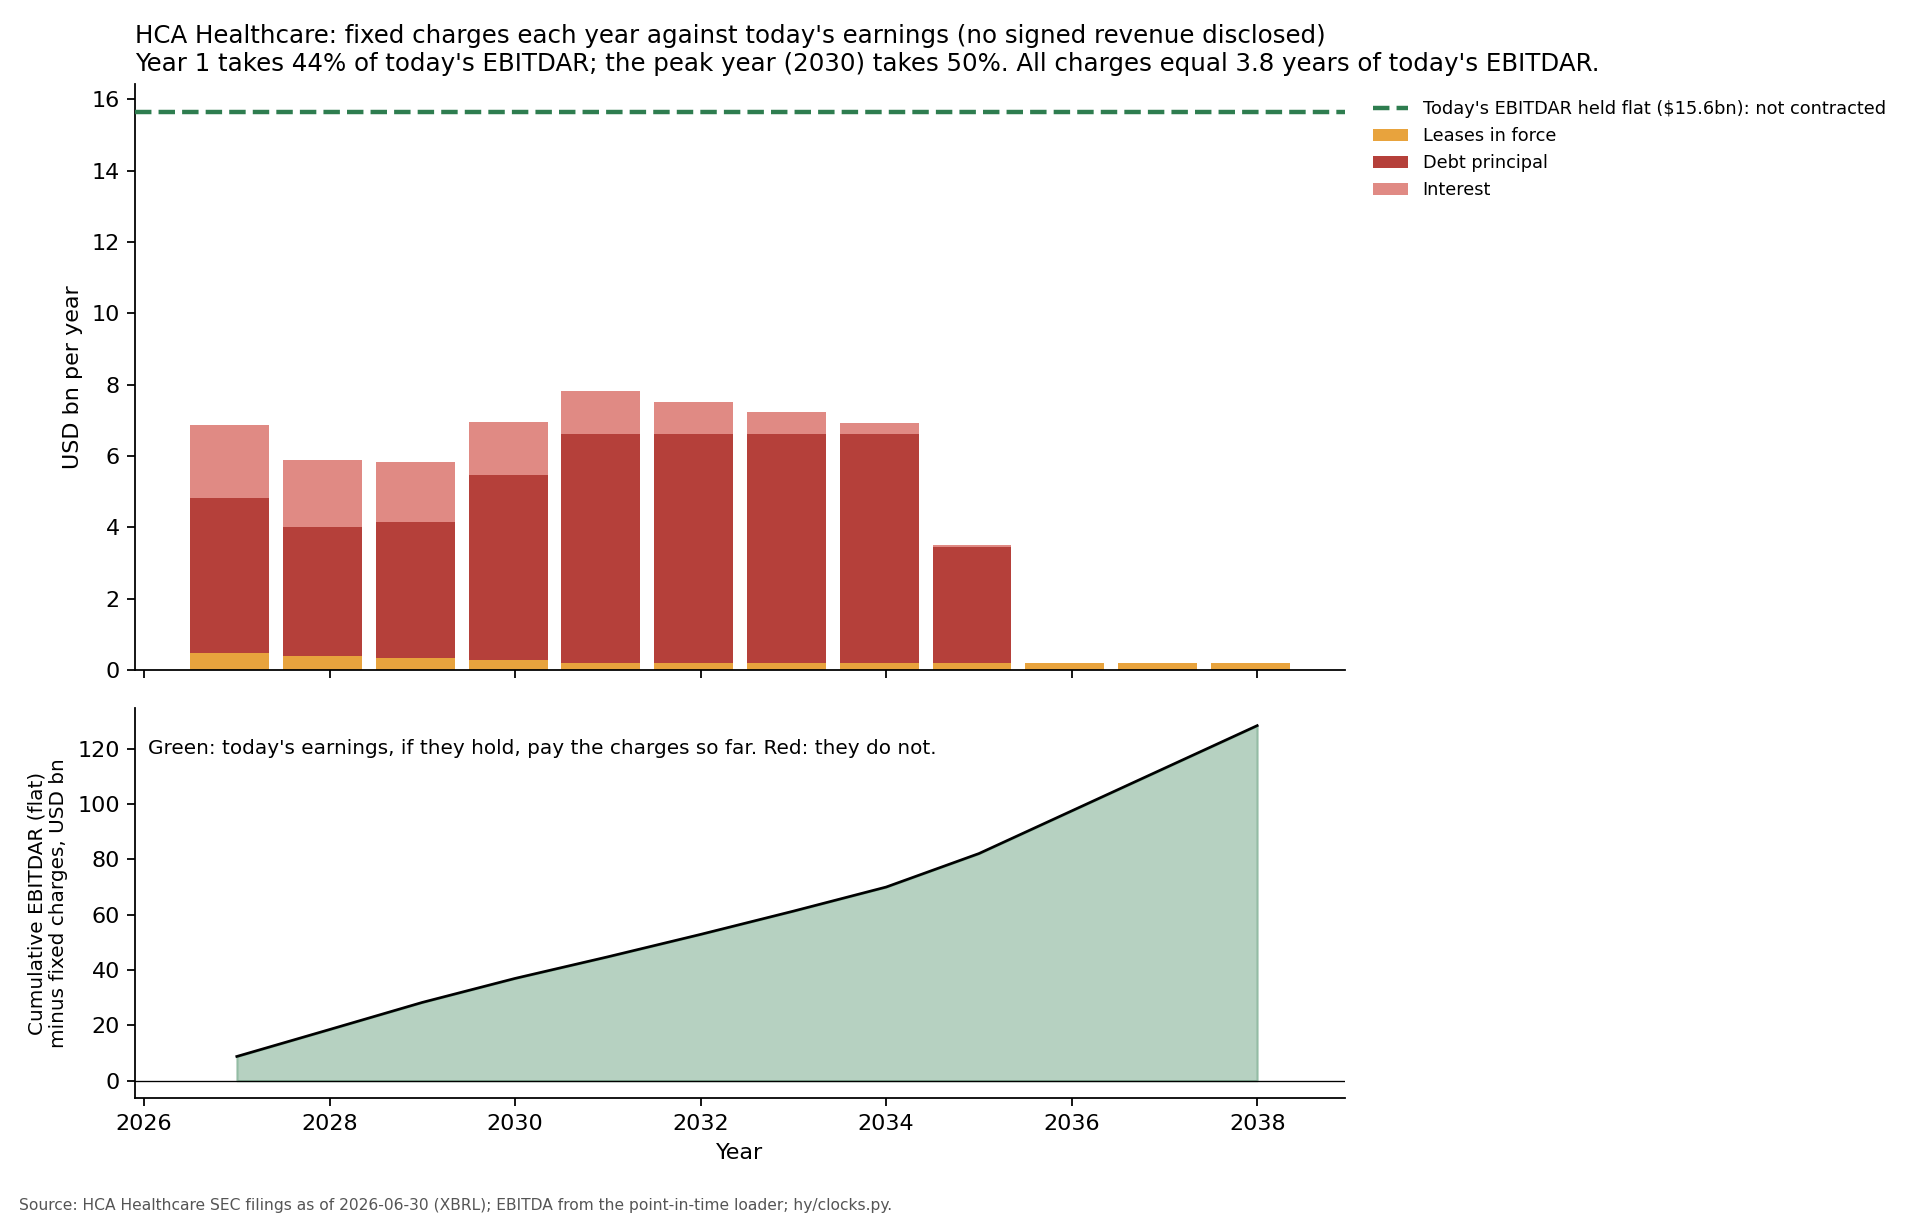
\includegraphics[width=\linewidth]{figures/clocks_all_HCA.png}\end{figure}
\begin{itemize}
\item \textbf{Fixed charges:} \$59bn, centred on year 4.4. That is 3.8 years of today's EBITDAR.
\item \textbf{No contract clock} (no signed revenue disclosed). The green line is today's EBITDAR held flat, not a contract.
\item \textbf{Debt schedule:} ladder short of balance-sheet debt by 32,038; residual put in 'thereafter'; balance-sheet debt 45,828 (tag LongTermDebt).
\end{itemize}\newpage
\section*{HCA Healthcare (HCA): scenarios under each macro path}
\begin{figure}[H]\centering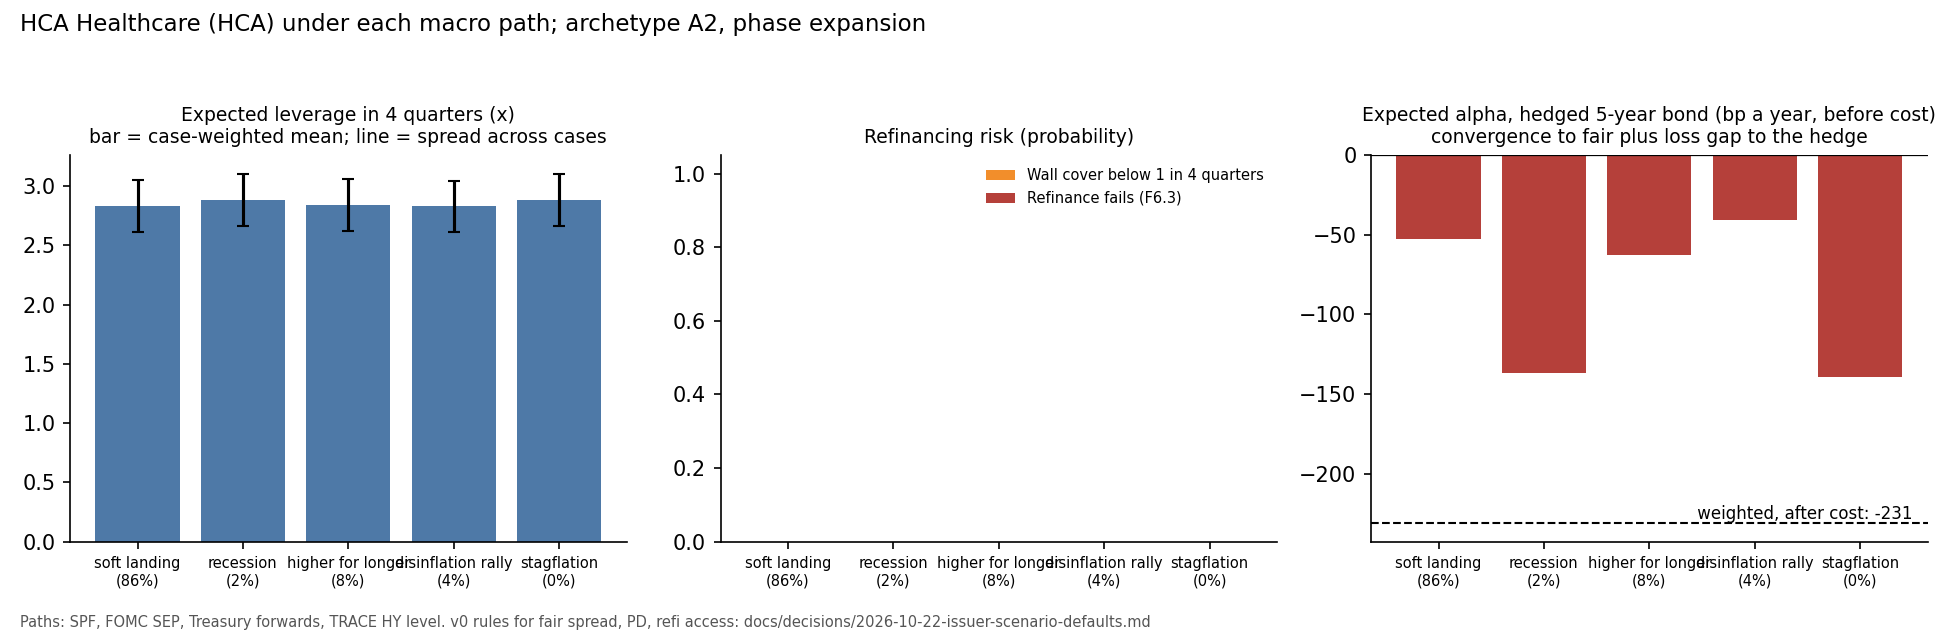
\includegraphics[width=\linewidth]{figures/scenarios_HCA.png}\end{figure}
\begin{center}\footnotesize\setlength{\tabcolsep}{4pt}
\begin{tabular}{@{}lrrrrrrrr@{}}\toprule
Path & Prob. & Lev. 4q & Peak lev. (down) & F4 score & Wall risk & Refi fails & PD 12m & Alpha (bp/yr) \\\midrule
soft landing & 86\% & 2.8x & 3.9x & 4 & 0\% & 0\% & 0.6\% & -50 \\
recession & 2\% & 2.9x & 4.0x & 3 & 0\% & 0\% & 1.6\% & -129 \\
higher for longer & 8\% & 2.8x & 3.9x & 4 & 0\% & 0\% & 0.7\% & -59 \\
disinflation rally & 4\% & 2.8x & 3.9x & 4 & 0\% & 0\% & 0.5\% & -39 \\
stagflation & 0\% & 2.9x & 4.0x & 3 & 0\% & 0\% & 1.6\% & -131 \\
\bottomrule
\end{tabular}
\end{center}
\begin{itemize}
\item \textbf{Weighted expected alpha}, hedged 5-year bond, 6-month horizon: -52 bp a year before cost, -228 bp after a 20 bp bid-ask round trip. Framework F9 G3 (alpha after cost above zero): fails.
\item \textbf{Inputs}: archetype A2; 5-year spread 68 bp against a fair 88 bp (pair report fair line); starting growth 1.6\% a quarter; 6,192 of 45,828 (USD m) of debt due inside 8 quarters. F4 points held on every path: rating proxy, recent raise.
\item \textbf{Read with care}: fair spread, default probability, and refinance access follow the v0 rules of \texttt{docs/decisions/2026-10-22-issuer-scenario-defaults.md}. Under spread-proportional pricing a mispricing scales with the market, so the stress paths enlarge it; real stress often widens a gap before it closes.
\end{itemize}
\newpage
\section{Tenet Healthcare (THC), filing of 2026-06-30}
\begin{figure}[H]\centering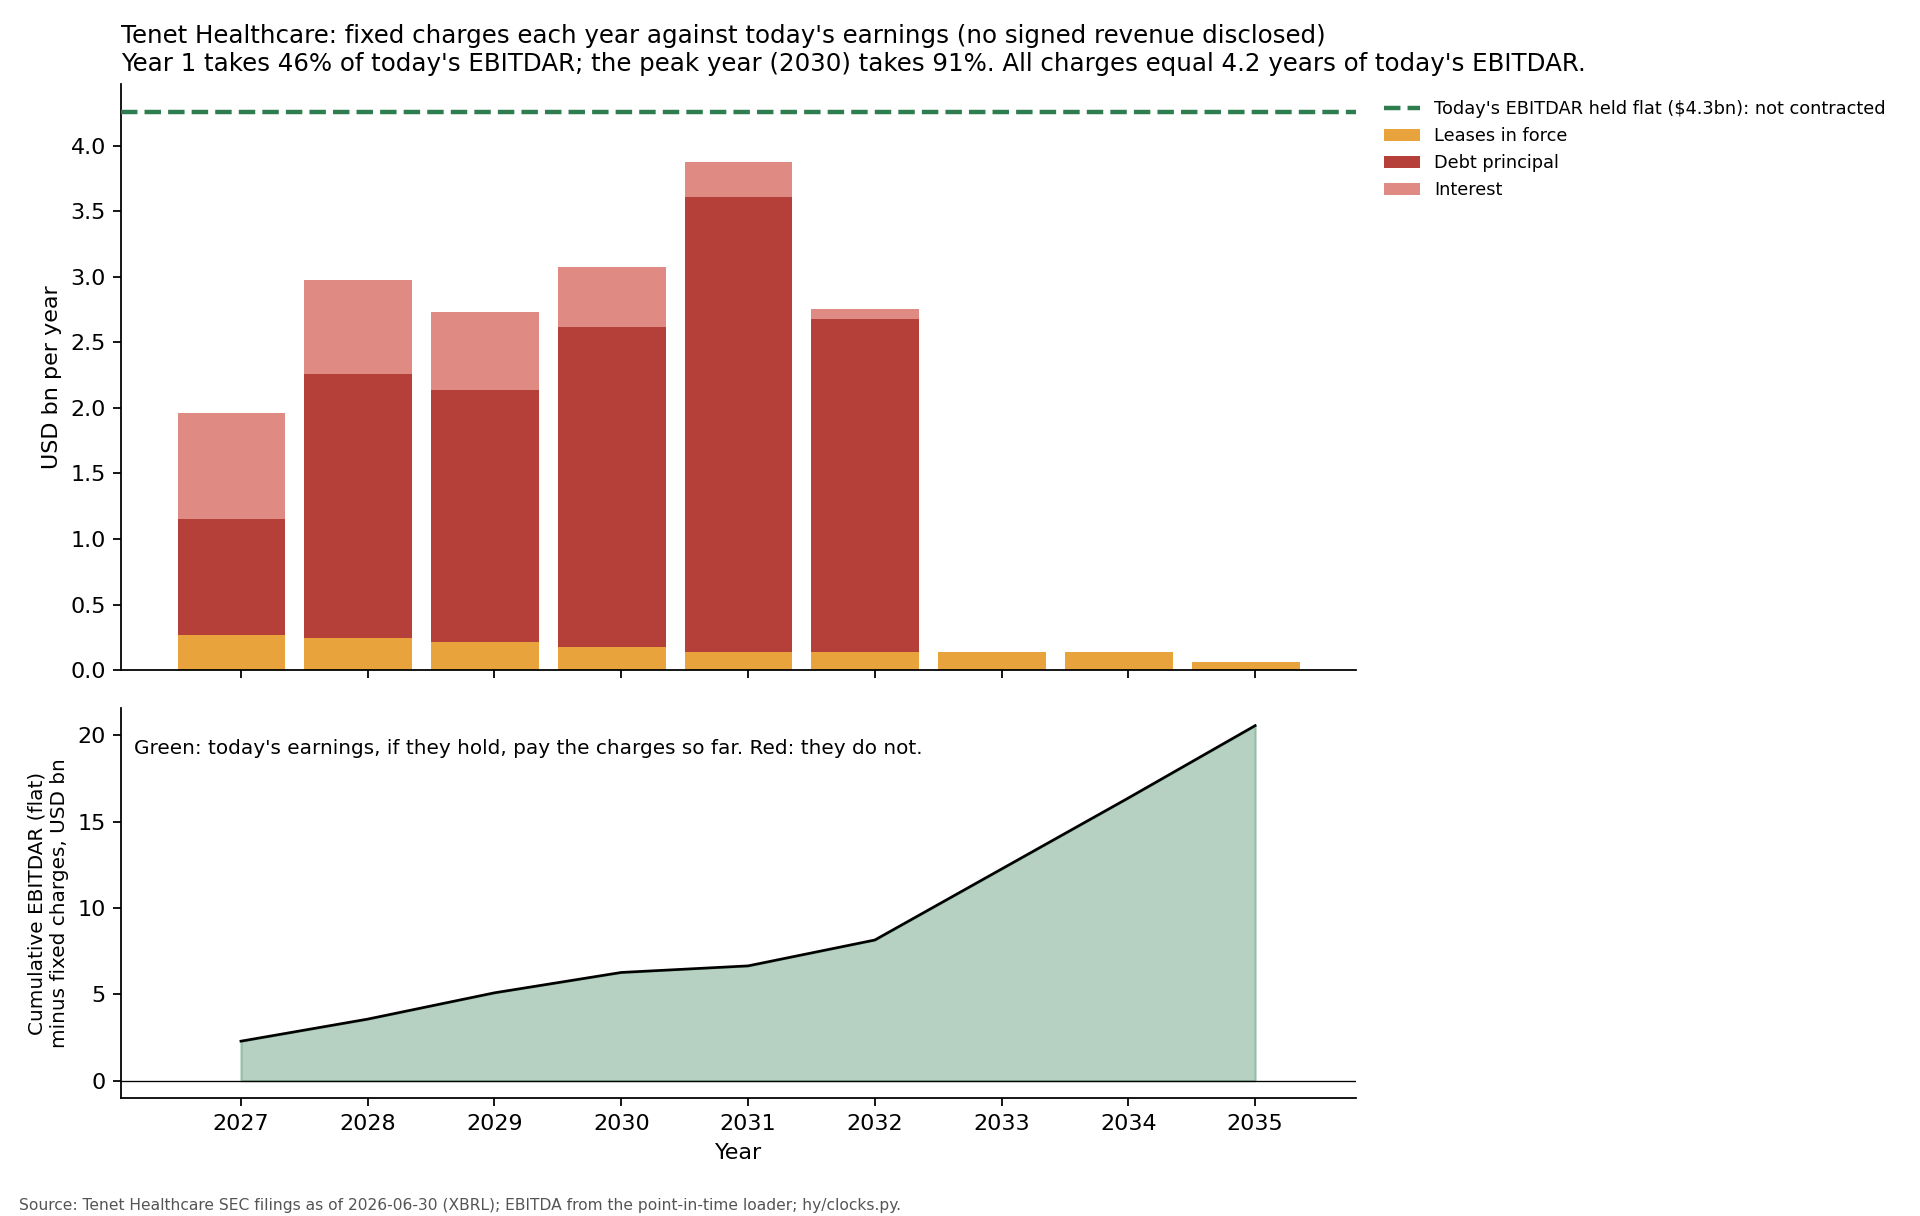
\includegraphics[width=\linewidth]{figures/clocks_all_THC.png}\end{figure}
\begin{itemize}
\item \textbf{Fixed charges:} \$18bn, centred on year 3.3. That is 4.2 years of today's EBITDAR.
\item \textbf{No contract clock} (signed revenue under one year of sales). The green line is today's EBITDAR held flat, not a contract.
\item \textbf{Debt schedule:} ladder as filed; balance-sheet debt 13,248 (tag DebtAndCapitalLeaseObligations).
\end{itemize}\newpage
\section*{Tenet Healthcare (THC): scenarios under each macro path}
\begin{figure}[H]\centering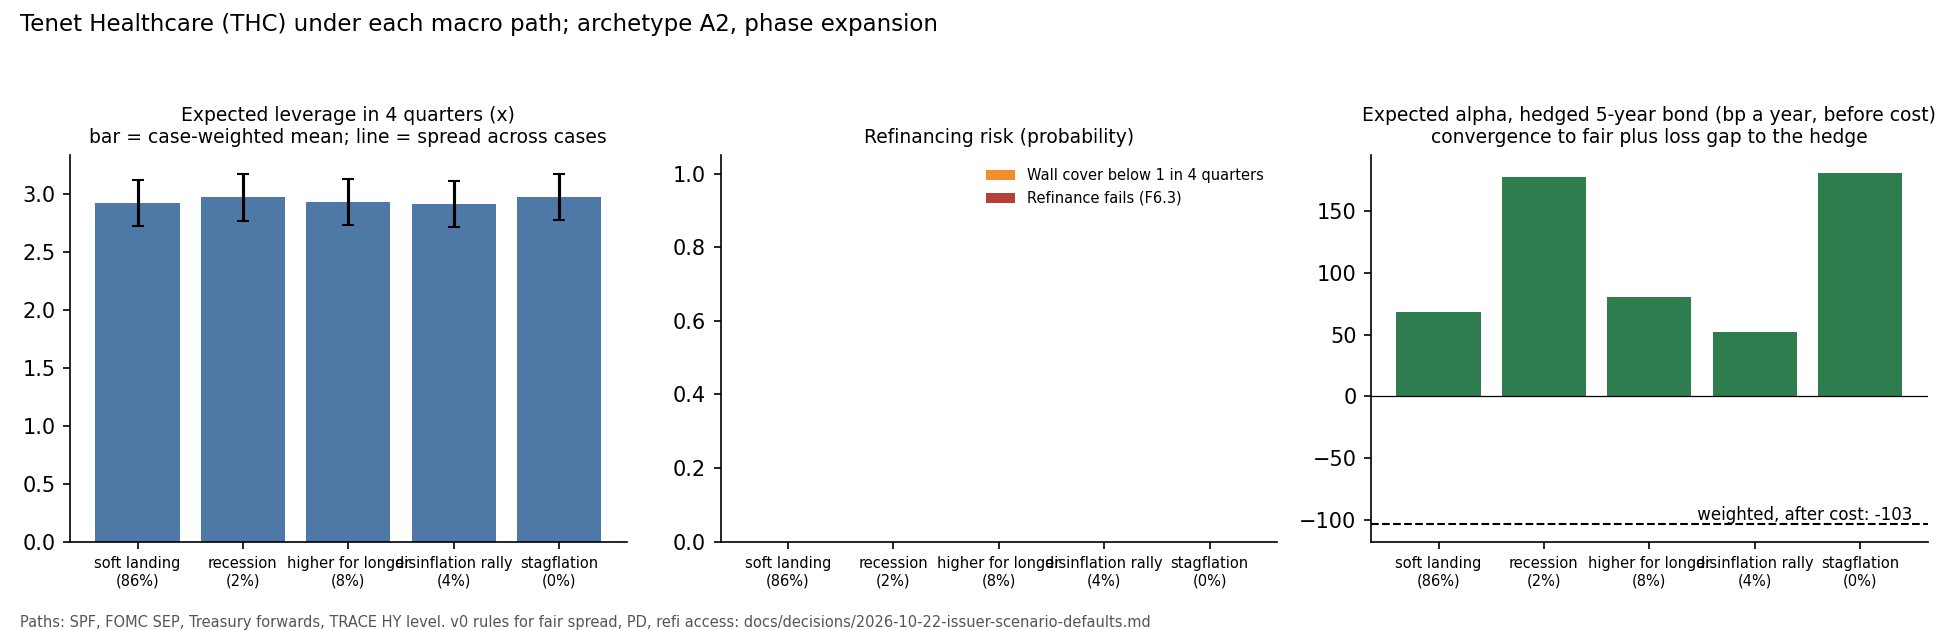
\includegraphics[width=\linewidth]{figures/scenarios_THC.png}\end{figure}
\begin{center}\footnotesize\setlength{\tabcolsep}{4pt}
\begin{tabular}{@{}lrrrrrrrr@{}}\toprule
Path & Prob. & Lev. 4q & Peak lev. (down) & F4 score & Wall risk & Refi fails & PD 12m & Alpha (bp/yr) \\\midrule
soft landing & 86\% & 2.9x & 4.0x & 3 & 0\% & 0\% & 0.7\% & +73 \\
recession & 2\% & 3.0x & 4.2x & 2 & 0\% & 0\% & 1.7\% & +191 \\
higher for longer & 8\% & 2.9x & 4.0x & 3 & 0\% & 0\% & 0.8\% & +87 \\
disinflation rally & 4\% & 2.9x & 3.9x & 3 & 0\% & 0\% & 0.5\% & +56 \\
stagflation & 0\% & 3.0x & 4.2x & 2 & 0\% & 0\% & 1.7\% & +194 \\
\bottomrule
\end{tabular}
\end{center}
\begin{itemize}
\item \textbf{Weighted expected alpha}, hedged 5-year bond, 6-month horizon: +76 bp a year before cost, -98 bp after a 20 bp bid-ask round trip. Framework F9 G3 (alpha after cost above zero): fails.
\item \textbf{Inputs}: archetype A2; 5-year spread 123 bp against a fair 93 bp (pair report fair line); starting growth 1.3\% a quarter; 1,707 of 13,248 (USD m) of debt due inside 8 quarters. F4 points held on every path: rating proxy.
\item \textbf{Read with care}: fair spread, default probability, and refinance access follow the v0 rules of \texttt{docs/decisions/2026-10-22-issuer-scenario-defaults.md}. Under spread-proportional pricing a mispricing scales with the market, so the stress paths enlarge it; real stress often widens a gap before it closes.
\end{itemize}
\newpage
\section{Carnival Corp (CCL), filing of 2026-05-31}
\begin{figure}[H]\centering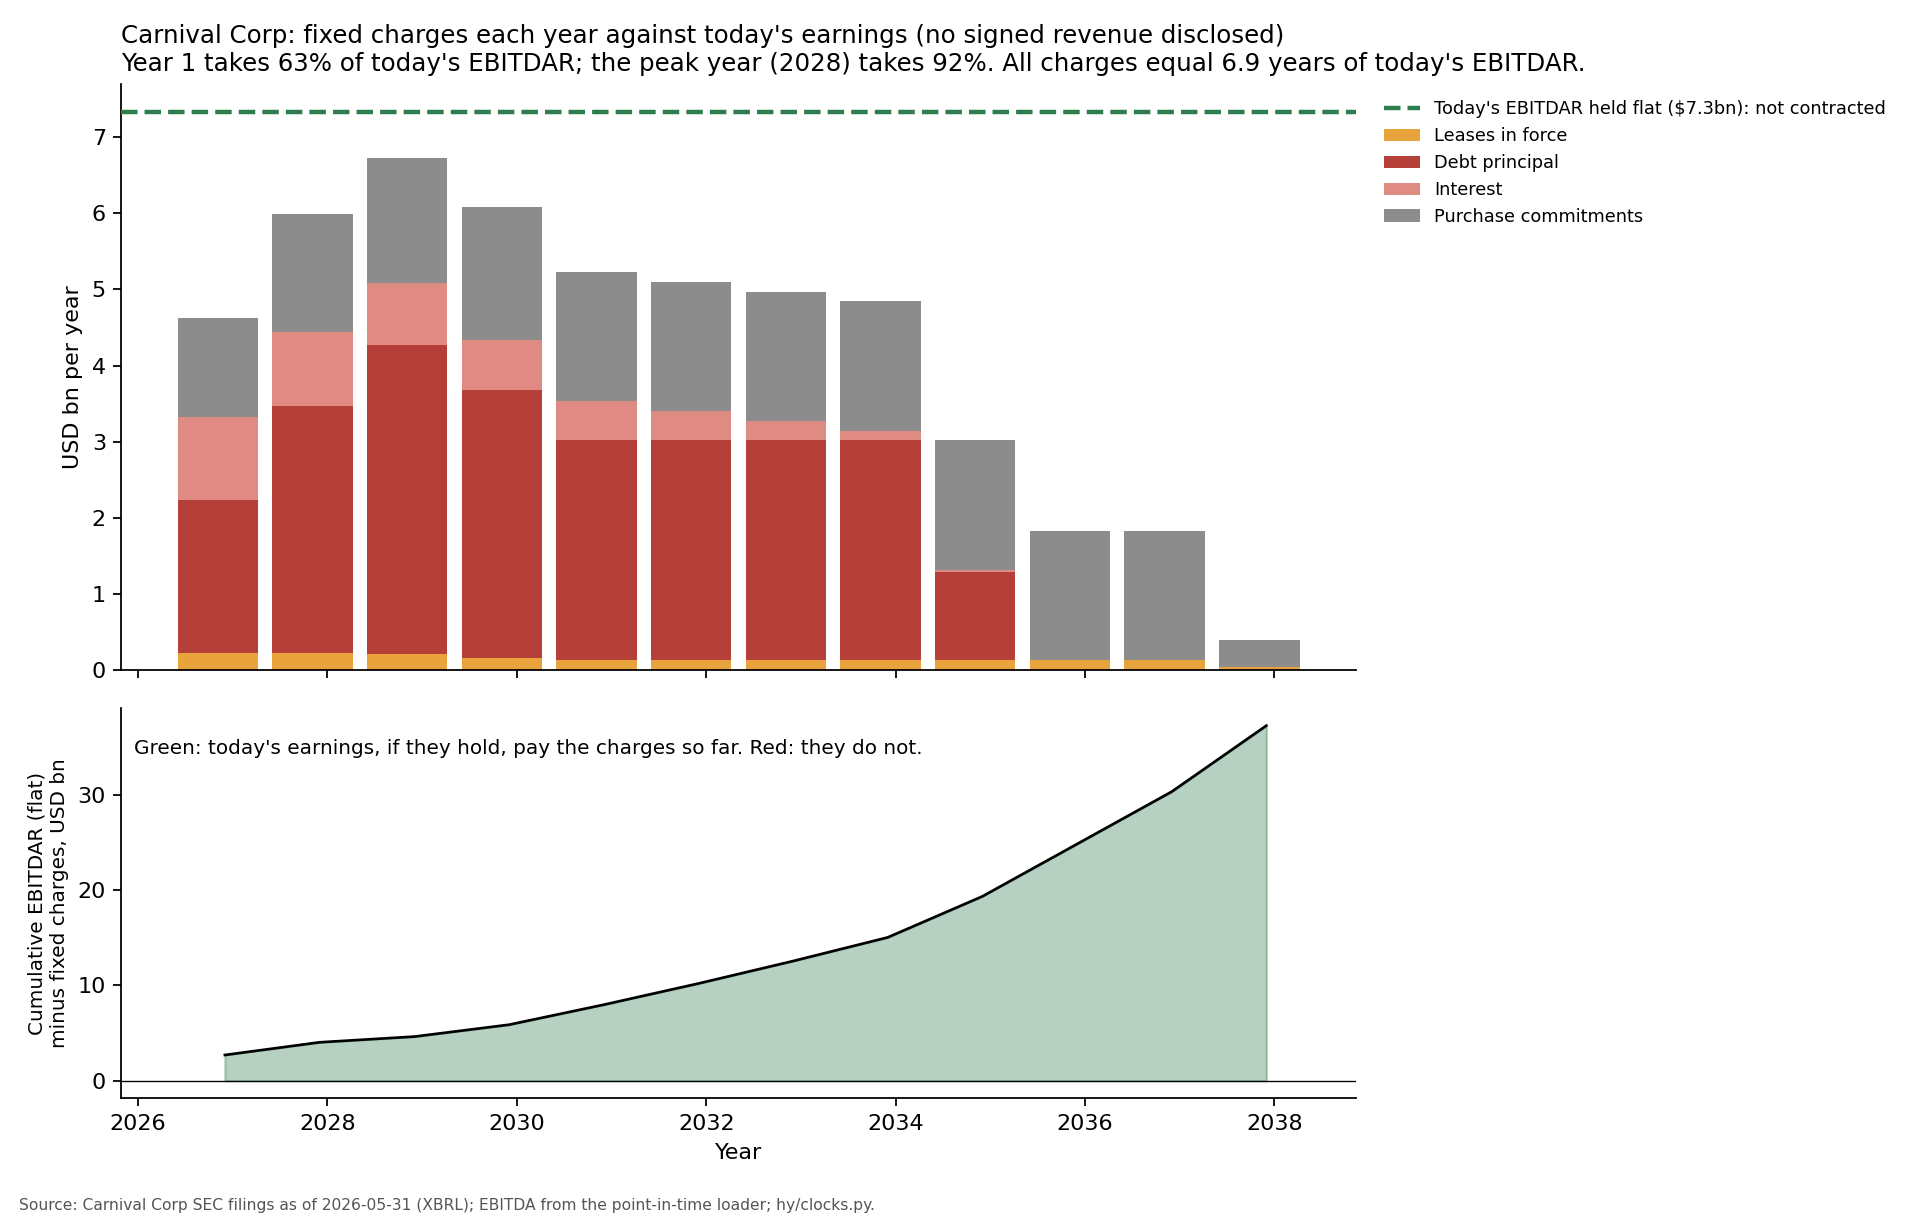
\includegraphics[width=\linewidth]{figures/clocks_all_CCL.png}\end{figure}
\begin{itemize}
\item \textbf{Fixed charges:} \$51bn, centred on year 4.7. That is 6.9 years of today's EBITDAR.
\item \textbf{No contract clock} (no signed revenue disclosed). The green line is today's EBITDAR held flat, not a contract.
\item \textbf{Debt schedule:} ladder as filed; balance-sheet debt 25,570 (tag LongTermDebt).
\end{itemize}\newpage
\section*{Carnival Corp (CCL): scenarios under each macro path}
\begin{figure}[H]\centering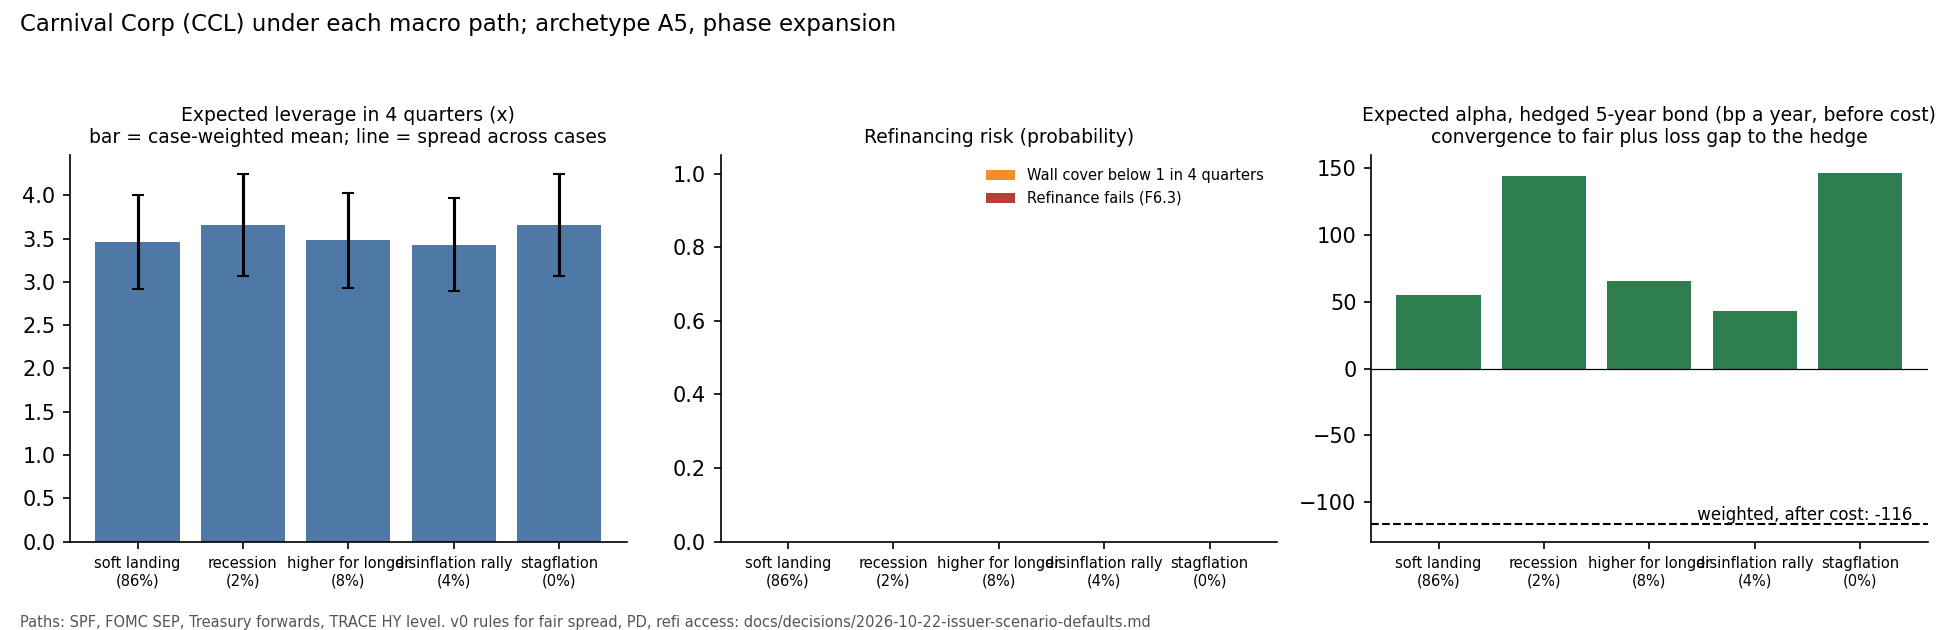
\includegraphics[width=\linewidth]{figures/scenarios_CCL.png}\end{figure}
\begin{center}\footnotesize\setlength{\tabcolsep}{4pt}
\begin{tabular}{@{}lrrrrrrrr@{}}\toprule
Path & Prob. & Lev. 4q & Peak lev. (down) & F4 score & Wall risk & Refi fails & PD 12m & Alpha (bp/yr) \\\midrule
soft landing & 86\% & 3.5x & 5.6x & 3 & 0\% & 0\% & 0.7\% & +59 \\
recession & 2\% & 3.7x & 5.9x & 2 & 0\% & 0\% & 1.9\% & +154 \\
higher for longer & 8\% & 3.5x & 5.6x & 3 & 0\% & 0\% & 0.9\% & +70 \\
disinflation rally & 4\% & 3.4x & 5.5x & 3 & 0\% & 0\% & 0.6\% & +46 \\
stagflation & 0\% & 3.7x & 5.9x & 2 & 0\% & 0\% & 1.9\% & +157 \\
\bottomrule
\end{tabular}
\end{center}
\begin{itemize}
\item \textbf{Weighted expected alpha}, hedged 5-year bond, 6-month horizon: +61 bp a year before cost, -112 bp after a 20 bp bid-ask round trip. Framework F9 G3 (alpha after cost above zero): fails.
\item \textbf{Inputs}: archetype A5; 5-year spread 129 bp against a fair 105 bp (pair report fair line); starting growth 1.3\% a quarter; 3,268 of 25,570 (USD m) of debt due inside 8 quarters. F4 points held on every path: rating proxy.
\item \textbf{Read with care}: fair spread, default probability, and refinance access follow the v0 rules of \texttt{docs/decisions/2026-10-22-issuer-scenario-defaults.md}. Under spread-proportional pricing a mispricing scales with the market, so the stress paths enlarge it; real stress often widens a gap before it closes.
\end{itemize}
\newpage
\section{Norwegian Cruise Line Holdings (NCLH), filing of 2026-06-30}
\begin{figure}[H]\centering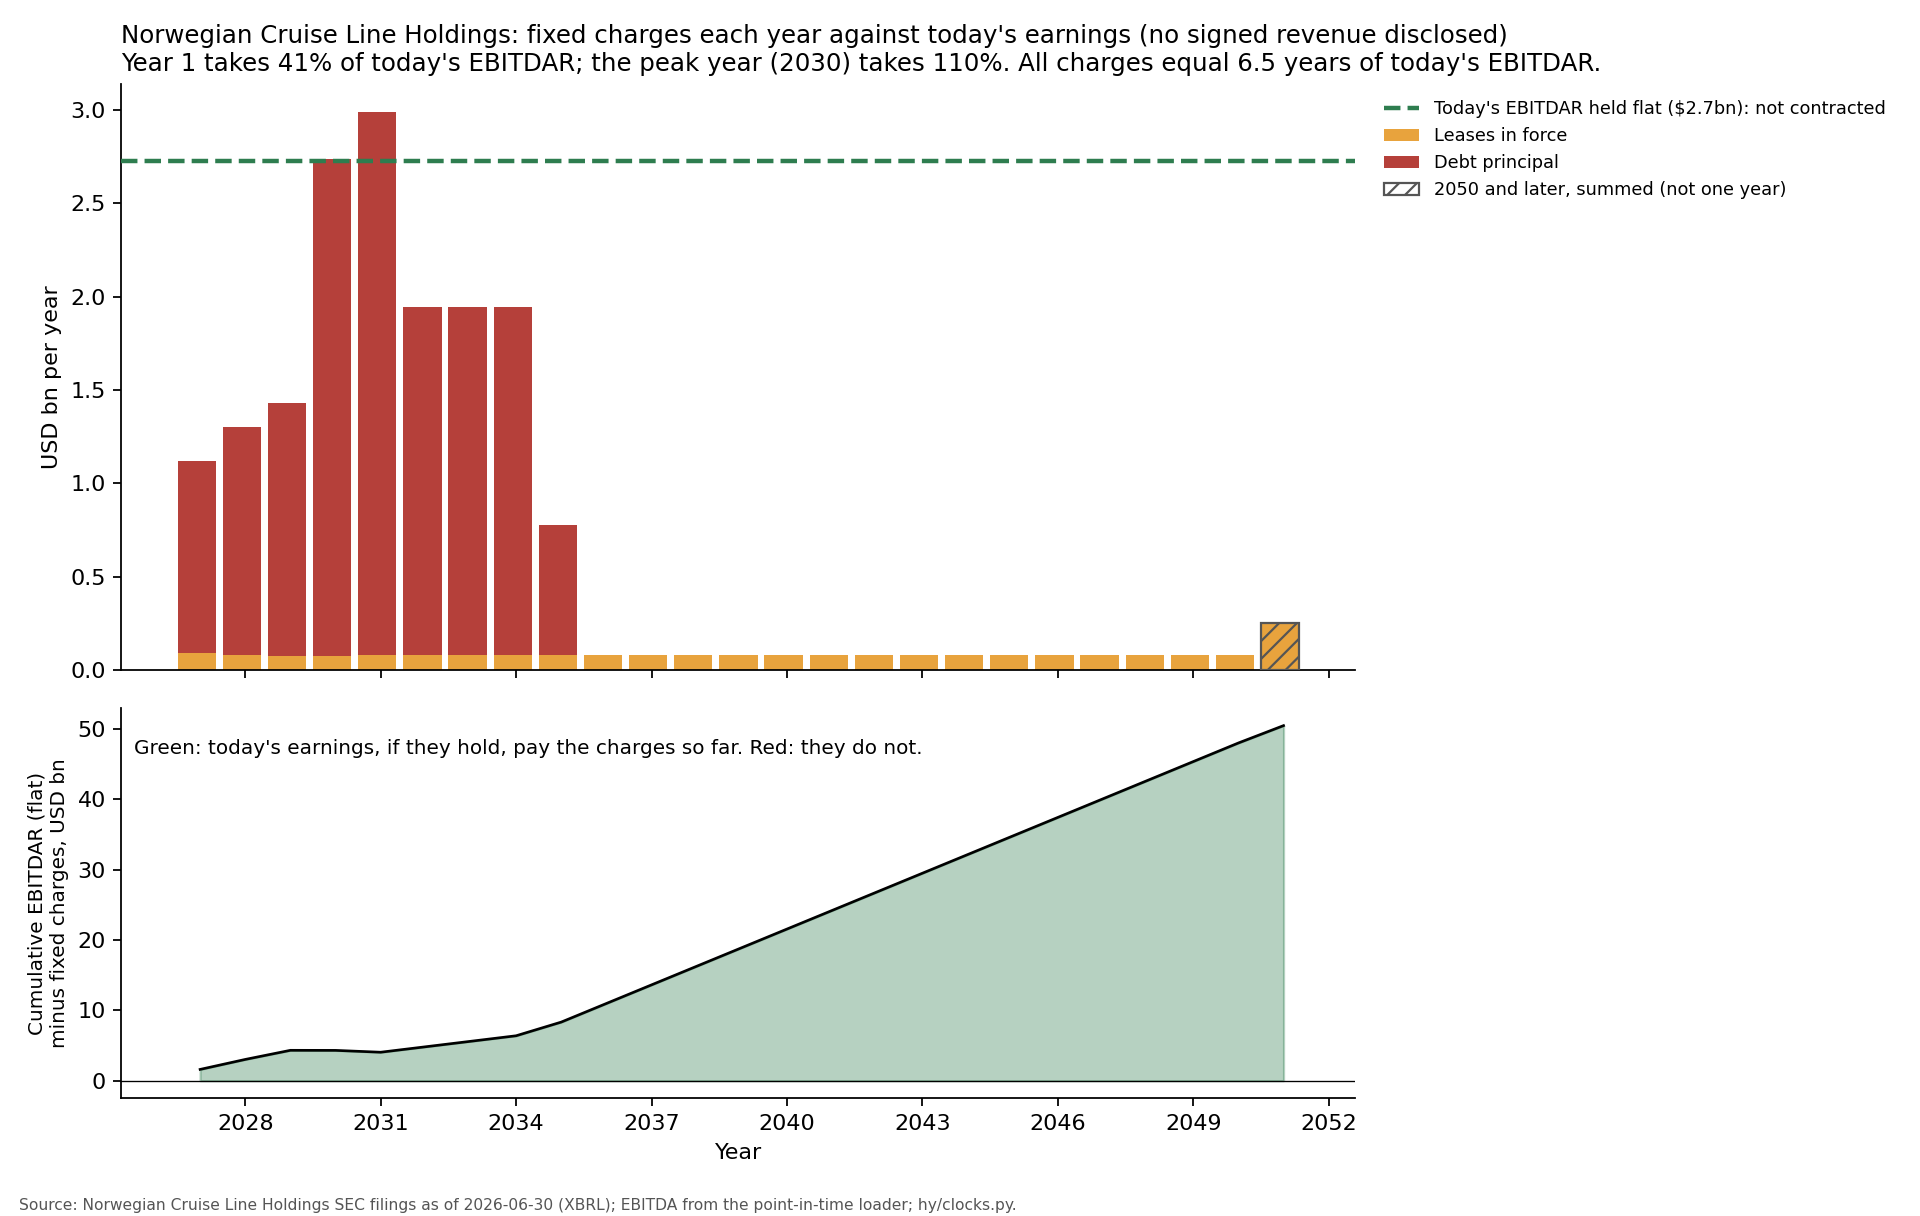
\includegraphics[width=\linewidth]{figures/clocks_all_NCLH.png}\end{figure}
\begin{itemize}
\item \textbf{Fixed charges:} \$18bn, centred on year 5.6. That is 6.5 years of today's EBITDAR.
\item \textbf{No contract clock} (no signed revenue disclosed). The green line is today's EBITDAR held flat, not a contract.
\item \textbf{Debt schedule:} ladder as filed; balance-sheet debt 15,468 (tag LongTermDebtAndCapitalLeaseObligationsIncludingCurrentMaturities).
\end{itemize}\newpage
\section*{Norwegian Cruise Line Holdings (NCLH): scenarios under each macro path}
\begin{figure}[H]\centering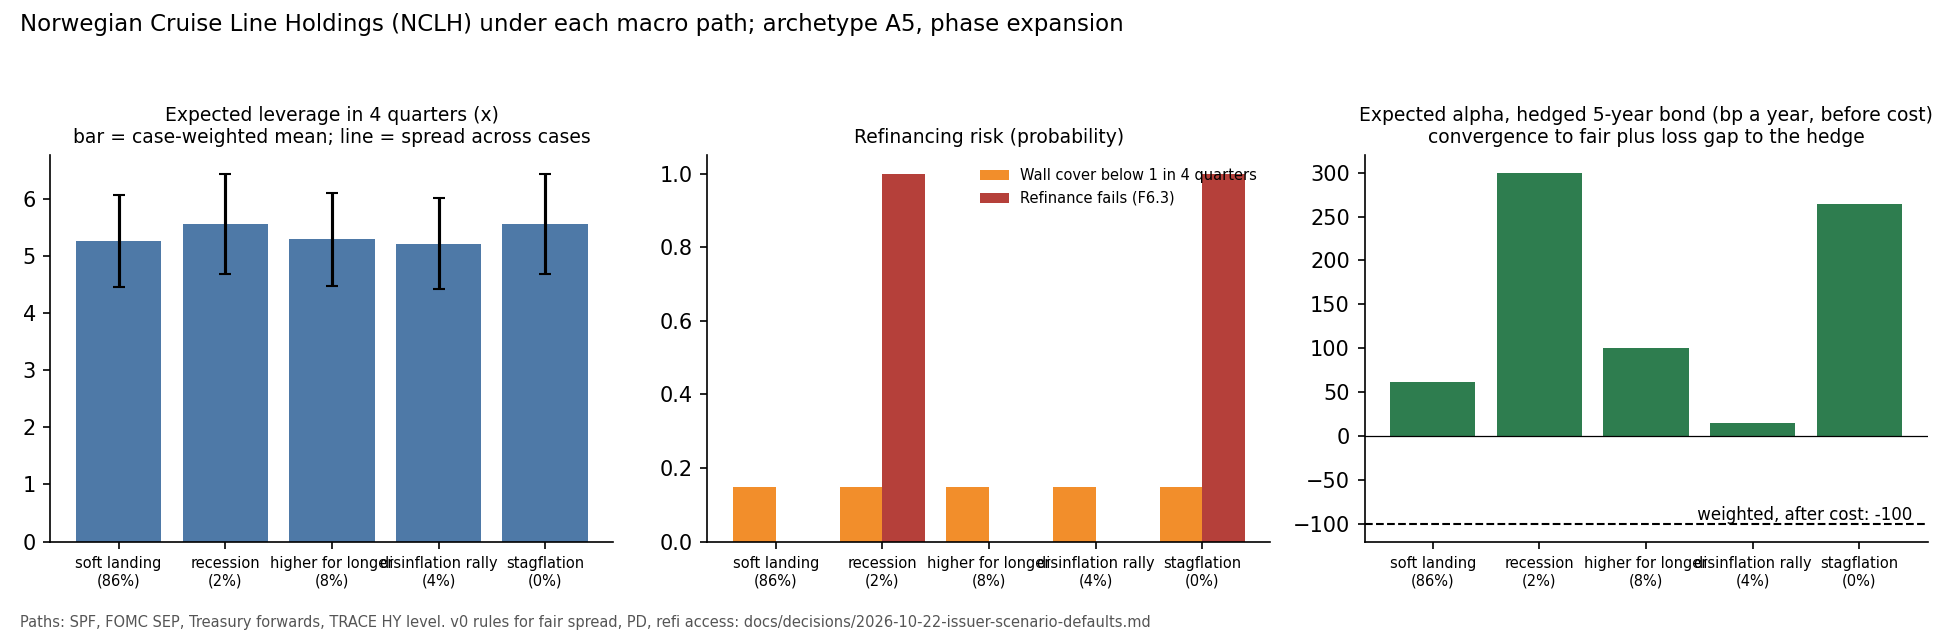
\includegraphics[width=\linewidth]{figures/scenarios_NCLH.png}\end{figure}
\begin{center}\footnotesize\setlength{\tabcolsep}{4pt}
\begin{tabular}{@{}lrrrrrrrr@{}}\toprule
Path & Prob. & Lev. 4q & Peak lev. (down) & F4 score & Wall risk & Refi fails & PD 12m & Alpha (bp/yr) \\\midrule
soft landing & 86\% & 5.3x & 8.6x & 3 & 15\% & 0\% & 2.3\% & +70 \\
recession & 2\% & 5.6x & 9.2x & 2 & 15\% & 100\% & 3.7\% & +314 \\
higher for longer & 8\% & 5.3x & 8.7x & 3 & 15\% & 0\% & 2.3\% & +109 \\
disinflation rally & 4\% & 5.2x & 8.6x & 3 & 15\% & 0\% & 2.3\% & +24 \\
stagflation & 0\% & 5.6x & 9.2x & 1 & 15\% & 100\% & 4.4\% & +282 \\
\bottomrule
\end{tabular}
\end{center}
\begin{itemize}
\item \textbf{Weighted expected alpha}, hedged 5-year bond, 6-month horizon: +77 bp a year before cost, -91 bp after a 20 bp bid-ask round trip. Framework F9 G3 (alpha after cost above zero): fails.
\item \textbf{Inputs}: archetype A5; 5-year spread 258 bp against a fair 208 bp (pair report fair line); starting growth 1.5\% a quarter; 1,584 of 15,468 (USD m) of debt due inside 8 quarters. F4 points held on every path: rating proxy.
\item \textbf{Read with care}: fair spread, default probability, and refinance access follow the v0 rules of \texttt{docs/decisions/2026-10-22-issuer-scenario-defaults.md}. Under spread-proportional pricing a mispricing scales with the market, so the stress paths enlarge it; real stress often widens a gap before it closes.
\end{itemize}
\newpage
\section{MGM Resorts International (MGM), filing of 2026-06-30}
\begin{figure}[H]\centering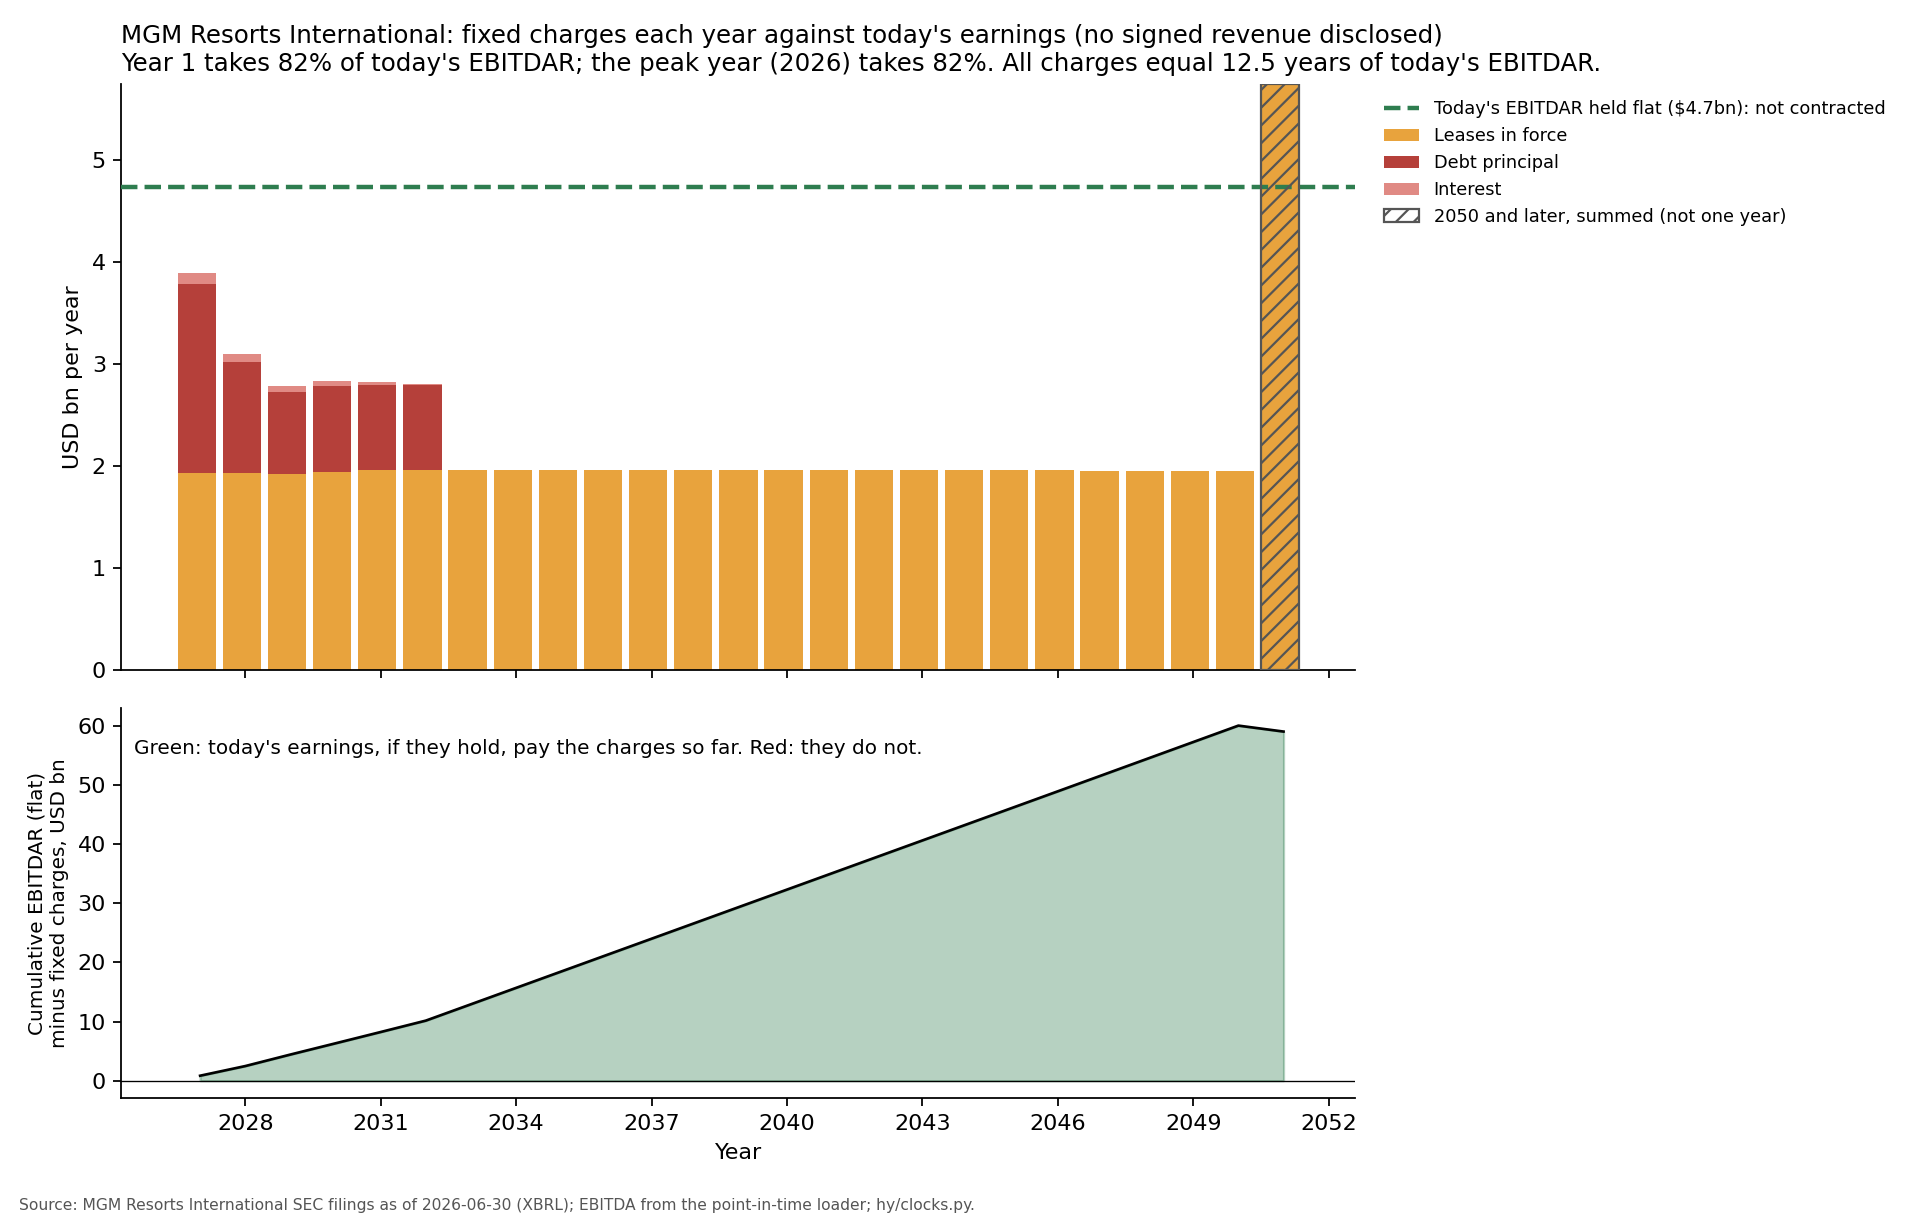
\includegraphics[width=\linewidth]{figures/clocks_all_MGM.png}\end{figure}
\begin{itemize}
\item \textbf{Fixed charges:} \$59bn, centred on year 12.2. That is 12.5 years of today's EBITDAR.
\item \textbf{No contract clock} (no signed revenue disclosed). The green line is today's EBITDAR held flat, not a contract.
\item \textbf{Debt schedule:} ladder as filed; balance-sheet debt 6,068 (tag LongTermDebt).
\end{itemize}\newpage
\section*{MGM Resorts International (MGM): scenarios under each macro path}
\begin{figure}[H]\centering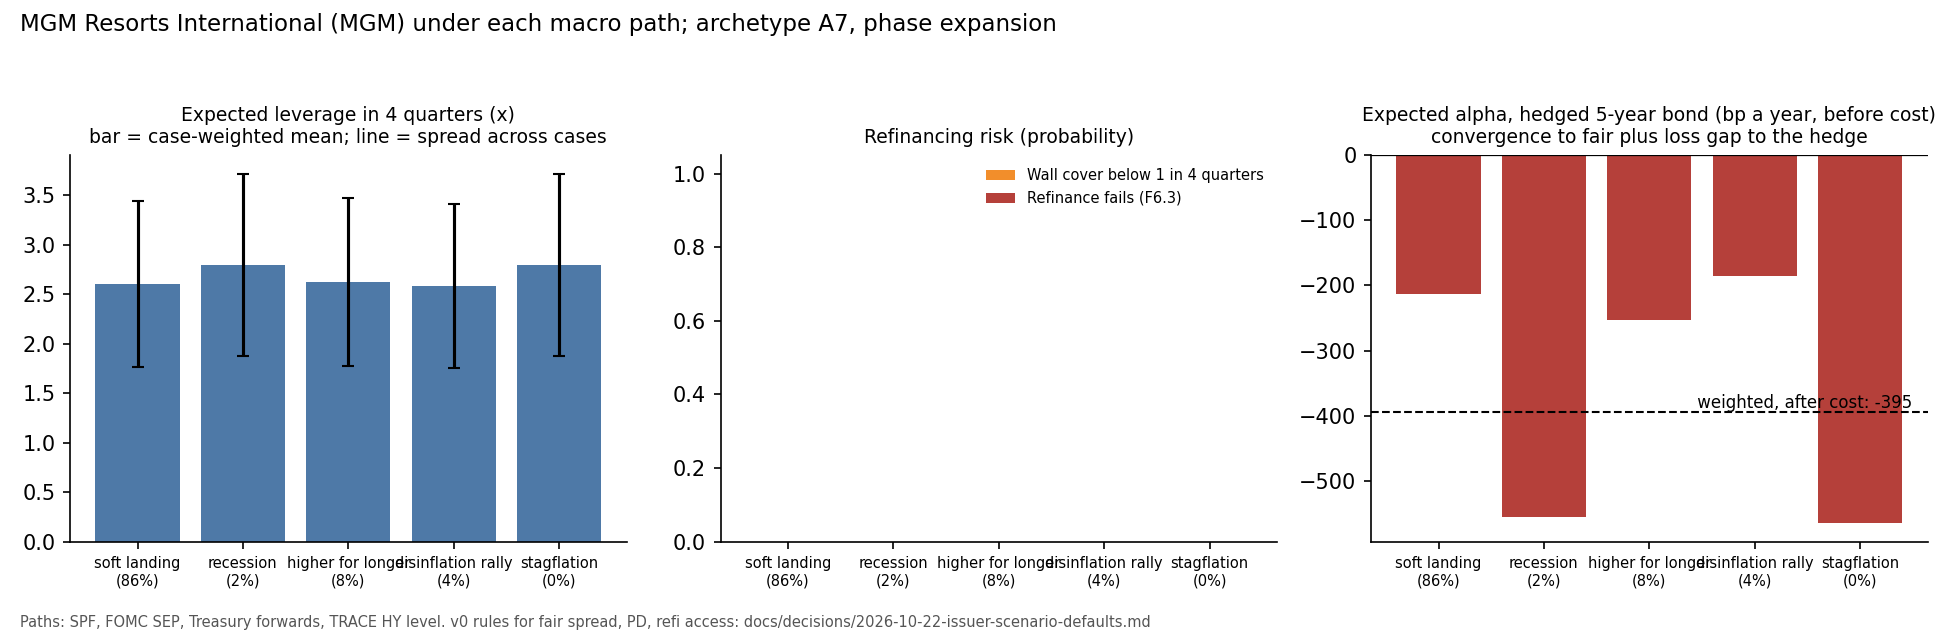
\includegraphics[width=\linewidth]{figures/scenarios_MGM.png}\end{figure}
\begin{center}\footnotesize\setlength{\tabcolsep}{4pt}
\begin{tabular}{@{}lrrrrrrrr@{}}\toprule
Path & Prob. & Lev. 4q & Peak lev. (down) & F4 score & Wall risk & Refi fails & PD 12m & Alpha (bp/yr) \\\midrule
soft landing & 86\% & 2.6x & 5.6x & 3 & 0\% & 0\% & 1.8\% & -203 \\
recession & 2\% & 2.8x & 6.1x & 2 & 0\% & 0\% & 4.6\% & -528 \\
higher for longer & 8\% & 2.6x & 5.7x & 3 & 0\% & 0\% & 2.1\% & -241 \\
disinflation rally & 4\% & 2.6x & 5.6x & 3 & 0\% & 0\% & 1.7\% & -176 \\
stagflation & 0\% & 2.8x & 6.1x & 2 & 0\% & 0\% & 4.7\% & -538 \\
\bottomrule
\end{tabular}
\end{center}
\begin{itemize}
\item \textbf{Weighted expected alpha}, hedged 5-year bond, 6-month horizon: -212 bp a year before cost, -384 bp after a 20 bp bid-ask round trip. Framework F9 G3 (alpha after cost above zero): fails.
\item \textbf{Inputs}: archetype A7; 5-year spread 175 bp against a fair 258 bp (pair report fair line); starting growth 0.8\% a quarter; 2,575 of 6,068 (USD m) of debt due inside 8 quarters. F4 points held on every path: rating proxy.
\item \textbf{Read with care}: fair spread, default probability, and refinance access follow the v0 rules of \texttt{docs/decisions/2026-10-22-issuer-scenario-defaults.md}. Under spread-proportional pricing a mispricing scales with the market, so the stress paths enlarge it; real stress often widens a gap before it closes.
\end{itemize}
\newpage
\section{Wynn Resorts (WYNN), filing of 2026-06-30}
\begin{figure}[H]\centering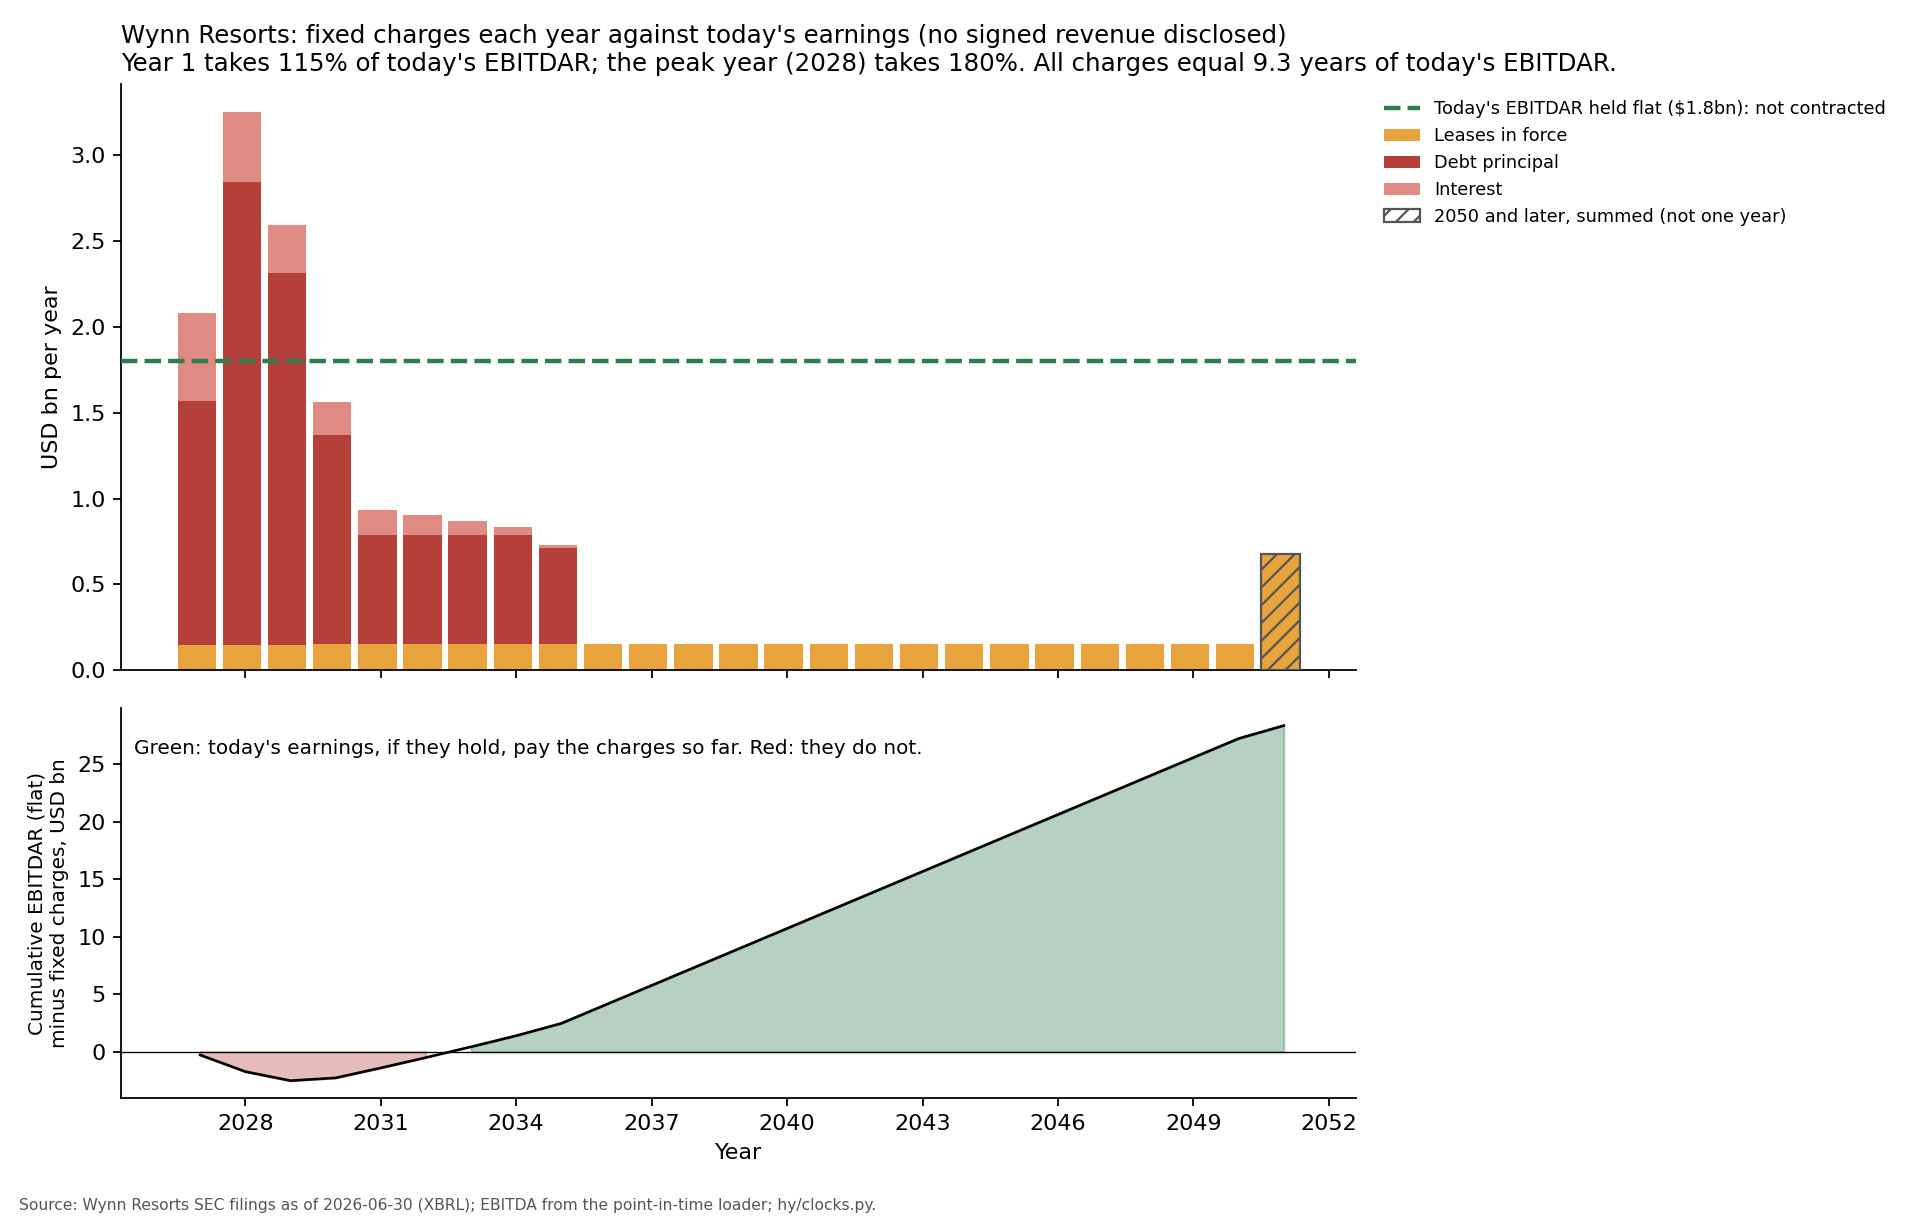
\includegraphics[width=\linewidth]{figures/clocks_all_WYNN.png}\end{figure}
\begin{itemize}
\item \textbf{Fixed charges:} \$17bn, centred on year 5.9. That is 9.3 years of today's EBITDAR.
\item \textbf{No contract clock} (no signed revenue disclosed). The green line is today's EBITDAR held flat, not a contract.
\item \textbf{Debt schedule:} ladder as filed; balance-sheet debt 10,725 (tag LongTermDebt).
\end{itemize}\newpage
\section*{Wynn Resorts (WYNN): scenarios under each macro path}
\begin{figure}[H]\centering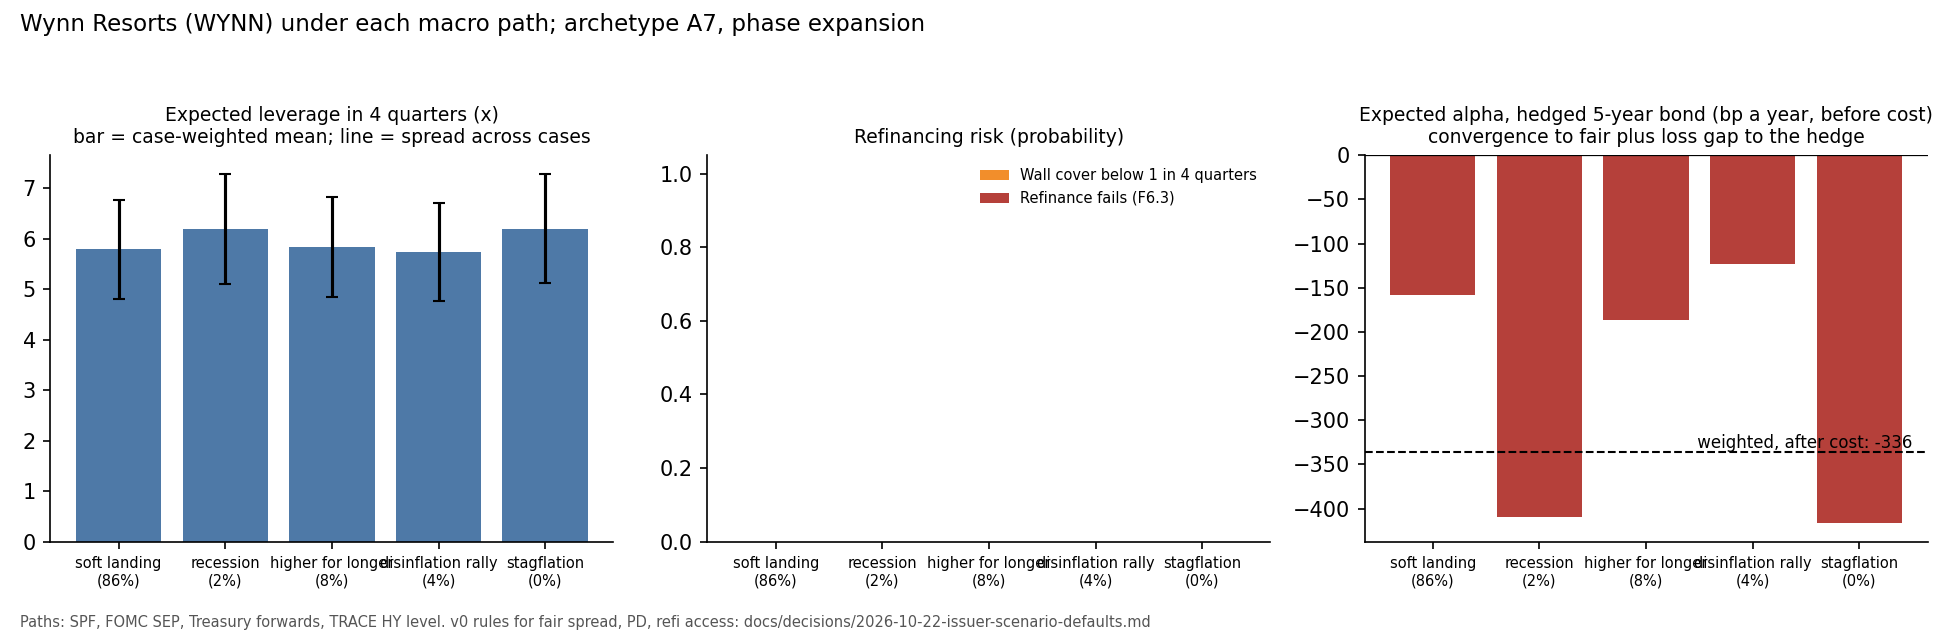
\includegraphics[width=\linewidth]{figures/scenarios_WYNN.png}\end{figure}
\begin{center}\footnotesize\setlength{\tabcolsep}{4pt}
\begin{tabular}{@{}lrrrrrrrr@{}}\toprule
Path & Prob. & Lev. 4q & Peak lev. (down) & F4 score & Wall risk & Refi fails & PD 12m & Alpha (bp/yr) \\\midrule
soft landing & 86\% & 5.8x & 9.3x & 3 & 0\% & 0\% & 1.6\% & -147 \\
recession & 2\% & 6.2x & 10.0x & 2 & 0\% & 0\% & 4.1\% & -382 \\
higher for longer & 8\% & 5.8x & 9.4x & 3 & 0\% & 0\% & 1.9\% & -174 \\
disinflation rally & 4\% & 5.7x & 9.2x & 3 & 0\% & 0\% & 1.2\% & -114 \\
stagflation & 0\% & 6.2x & 10.0x & 2 & 0\% & 0\% & 4.1\% & -389 \\
\bottomrule
\end{tabular}
\end{center}
\begin{itemize}
\item \textbf{Weighted expected alpha}, hedged 5-year bond, 6-month horizon: -153 bp a year before cost, -325 bp after a 20 bp bid-ask round trip. Framework F9 G3 (alpha after cost above zero): fails.
\item \textbf{Inputs}: archetype A7; 5-year spread 165 bp against a fair 226 bp (pair report fair line); starting growth 1.6\% a quarter; 2,868 of 10,725 (USD m) of debt due inside 8 quarters. F4 points held on every path: rating proxy.
\item \textbf{Read with care}: fair spread, default probability, and refinance access follow the v0 rules of \texttt{docs/decisions/2026-10-22-issuer-scenario-defaults.md}. Under spread-proportional pricing a mispricing scales with the market, so the stress paths enlarge it; real stress often widens a gap before it closes.
\end{itemize}
\newpage
\end{document}
